\documentclass[12pt,UTF8]{ctexart}
\usepackage{ctex,amsmath,amssymb,geometry,fancyhdr,bm,amsfonts
,mathtools,extarrows,graphicx,url,enumerate,color,float,multicol,rotating,subfig} 
\allowdisplaybreaks[4]
% 加入中文支持
\newcommand\Set[2]{\left\{#1\ \middle\vert\ #2 \right\}}
\newcommand\Lim[0]{\lim\limits_{n\rightarrow\infty}}
\newcommand\LIM[2]{\lim\limits_{#1\rightarrow#2}}
\newcommand\Ser[1]{\sum_{n=#1}^\infty}
\newcommand{\SER}[2]{\sum_{#1=#2}^\infty}
\newcommand{\Int}[4]{\int_{#1}^{#2}#3\mathrm d#4}
\geometry{a4paper,scale=0.80}
\pagestyle{fancy}
\rhead{多元函数微分学(2)}
\lhead{基础习题课期末复习}
\chead{微积分B(2)}
\begin{document}
\setcounter{section}{1}
\section{偏导数、全微分、复合函数微分法、隐函数微分法}
\noindent
\subsection{复习计划}
\begin{figure}[H]
\begin{center}
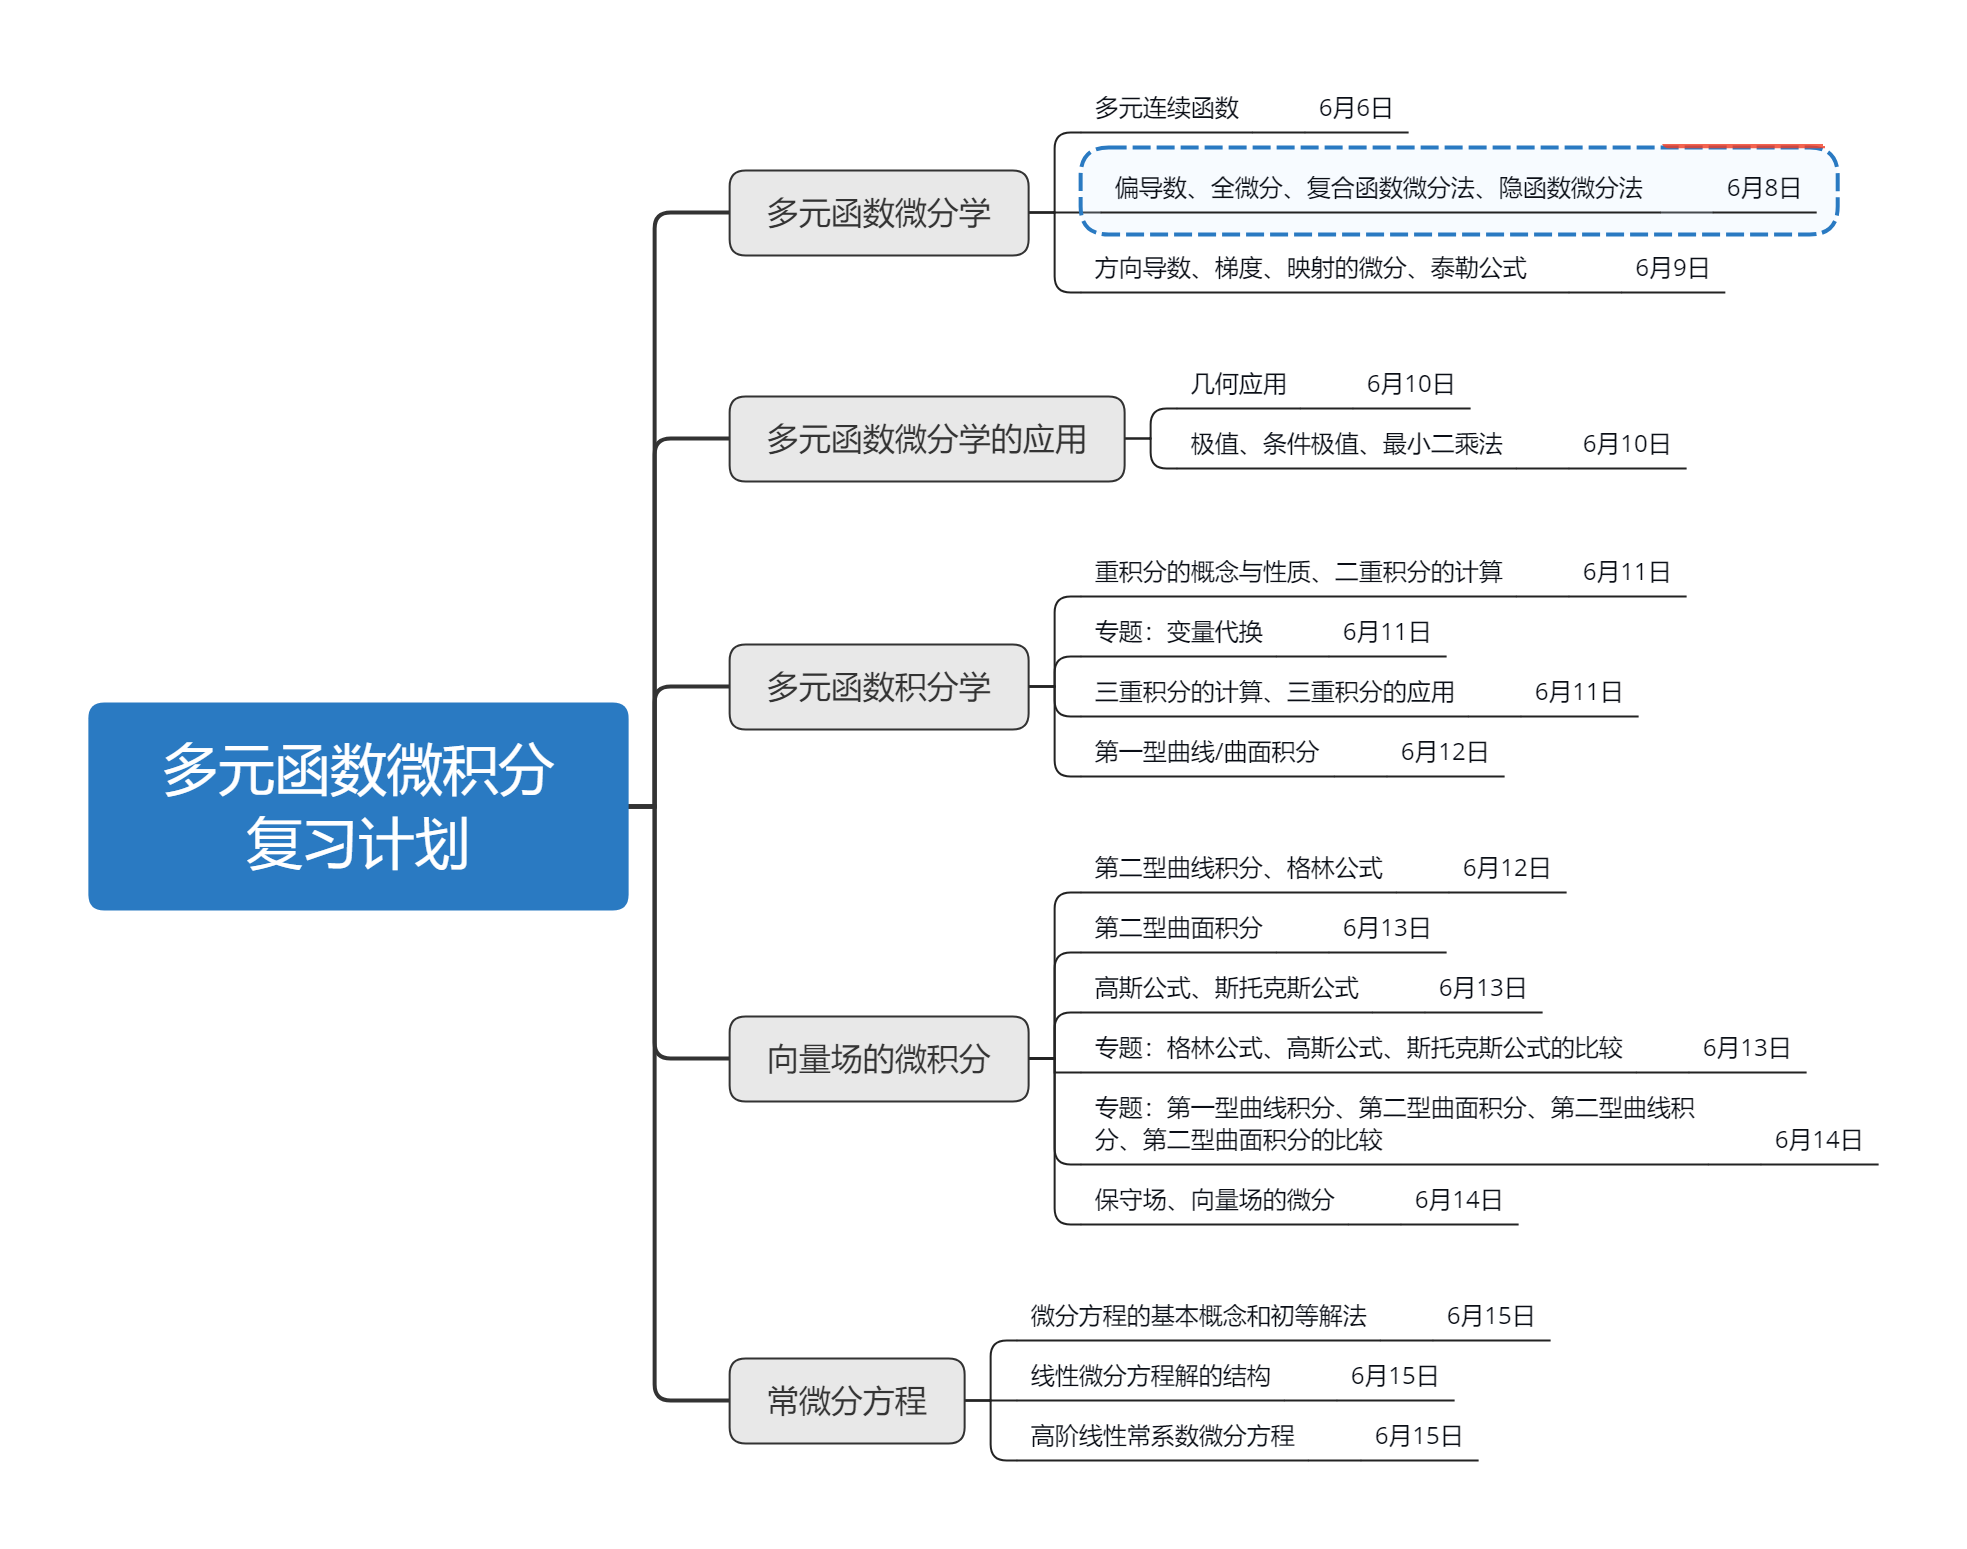
\includegraphics[height=0.5\textheight]{Figures20190607/plan.png}
\end{center}
\end{figure}
\subsection{知识结构}
\begin{figure}[H]
\begin{center}
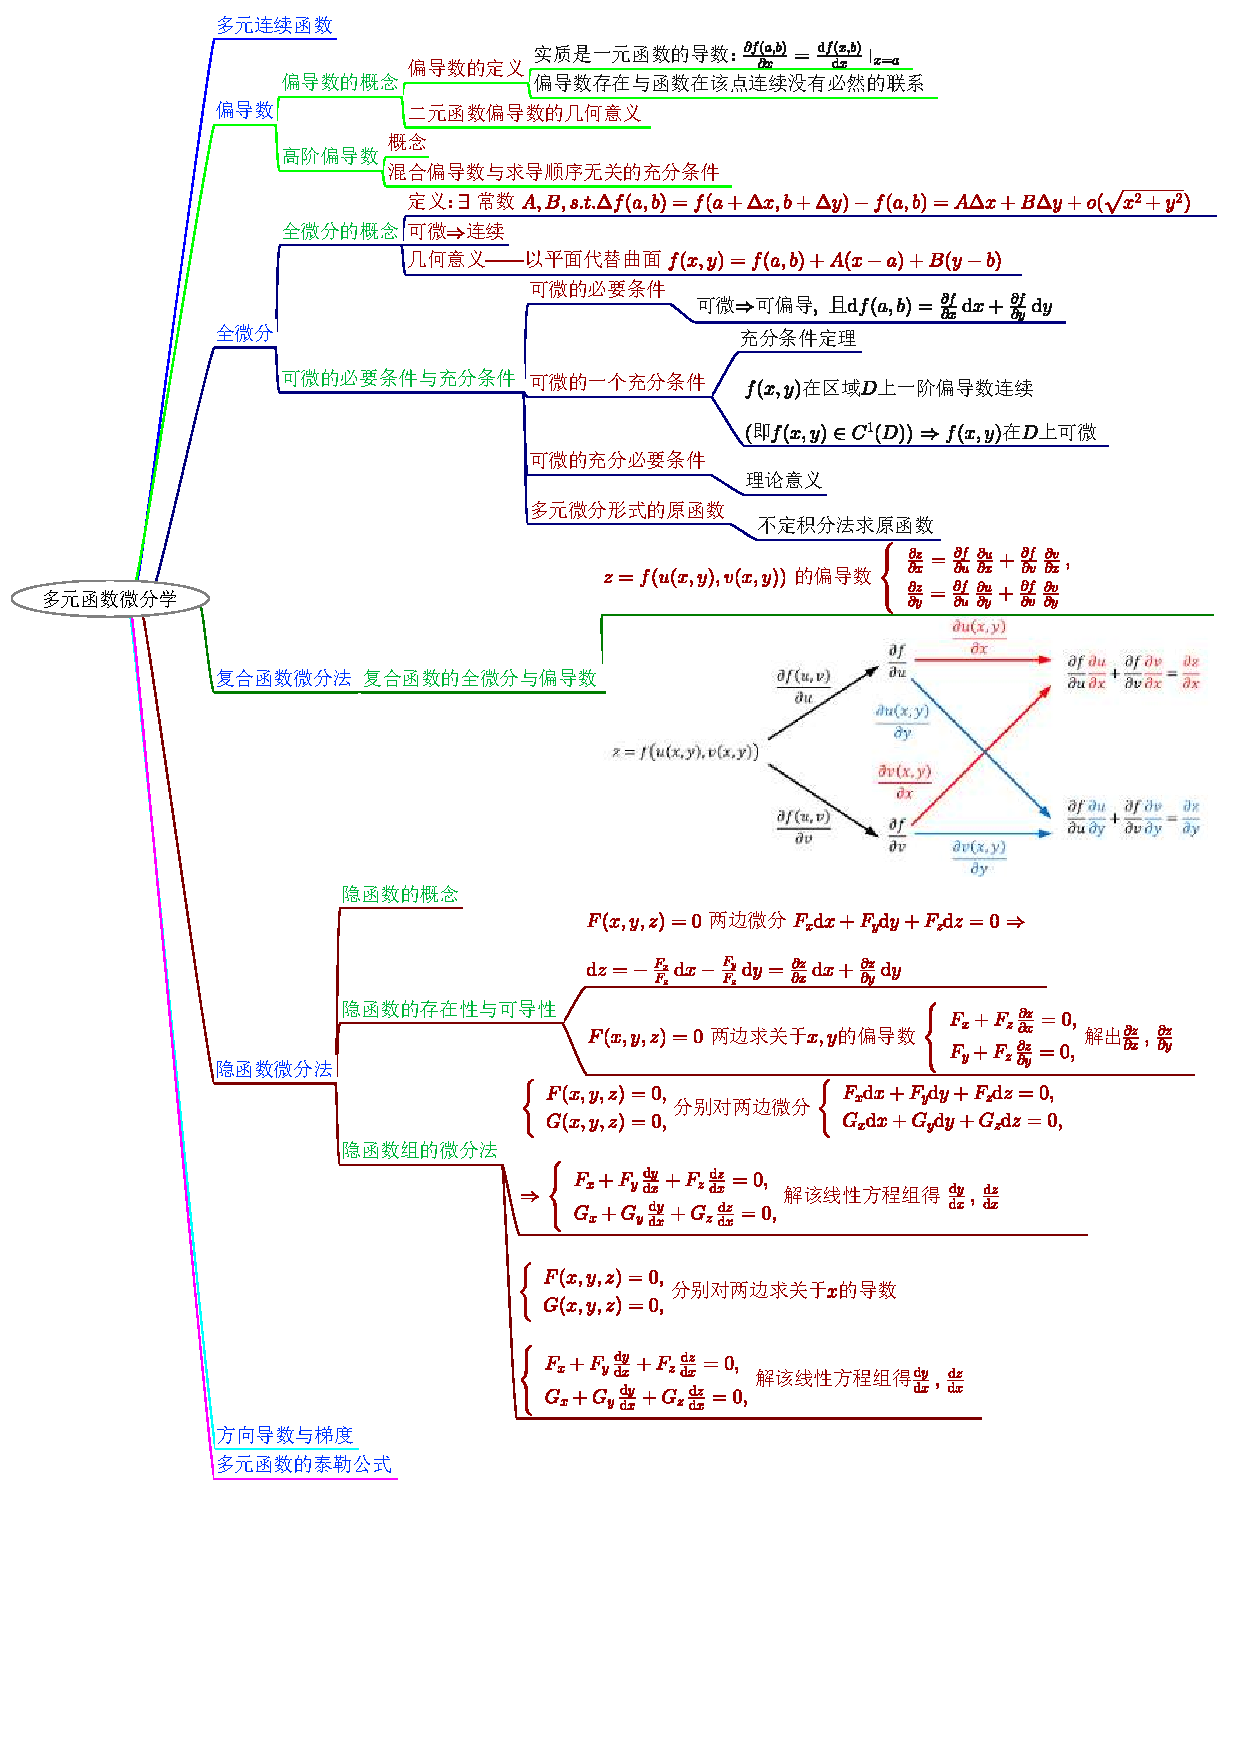
\includegraphics[height=0.9\textheight,angle=0]{20190607.pdf}
\end{center}
\end{figure}
\subsection{重要知识}
\begin{enumerate}
\item二元函数偏导数的几何意义
\begin{figure}[H]
\begin{center}
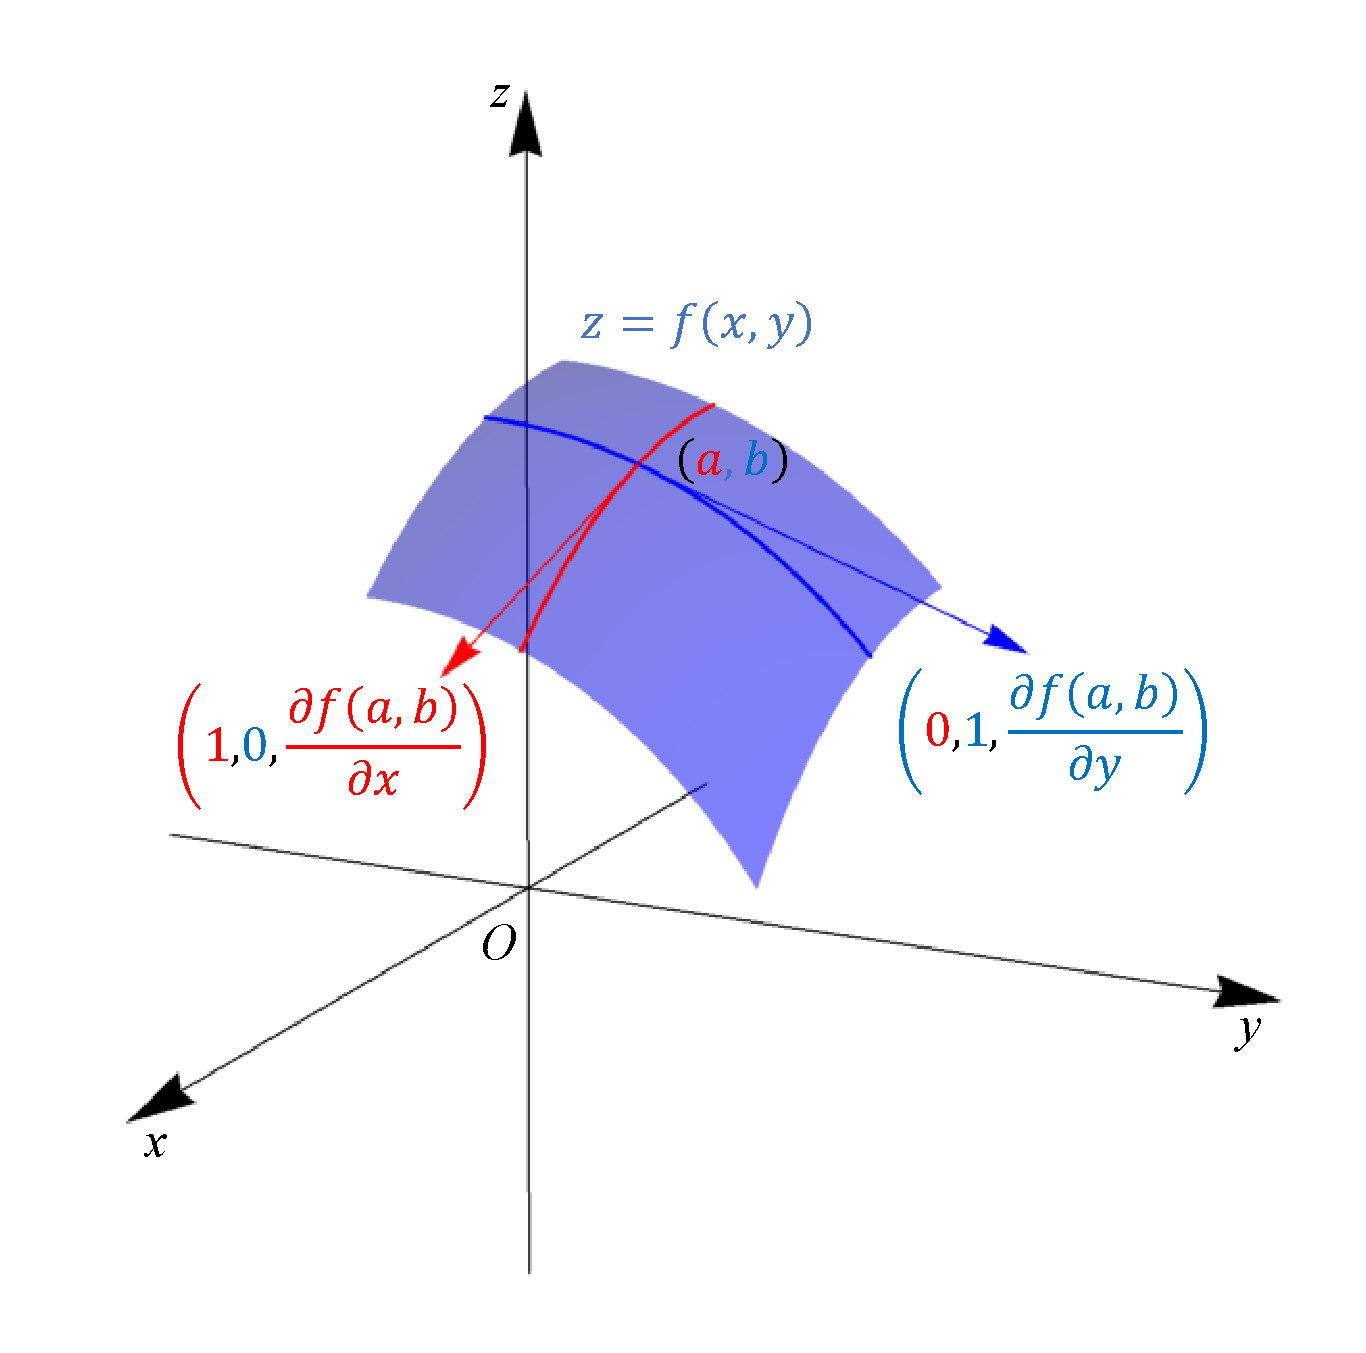
\includegraphics[height=0.5\textheight]{Figures20190607/partialderivative.pdf}
\end{center}
\caption{二元函数偏导数的几何意义}
\end{figure}
\item二元函数在一点连续、偏导数存在、可微及一阶偏导数连续之间的关系:
\begin{figure}[H]
\begin{center}
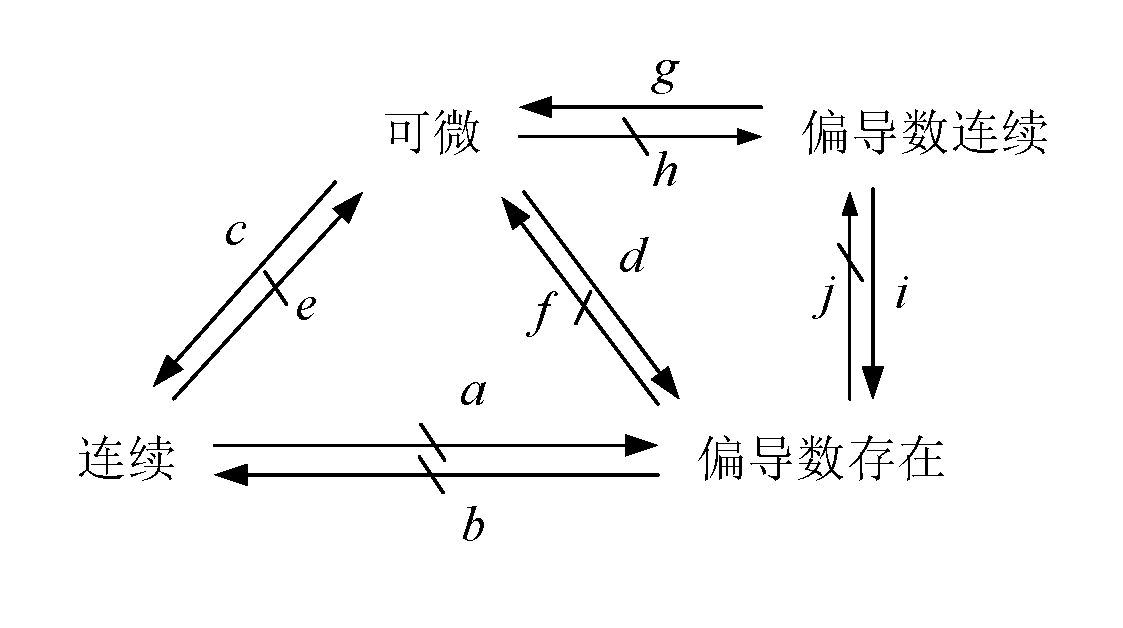
\includegraphics[height=0.2\textheight]{Figures20190607/relations.pdf}
\end{center}
\caption{二元函数在一点连续、偏导数存在、可微及一阶偏导数连续之间的关系}
\end{figure}
\begin{enumerate}
\item[a:]反例:函数$f(x,y)=\begin{cases}
\frac{xy}{x^2+y^2},&(x,y)\neq(0,0),\\
0,&(x,y)=(0,0),
\end{cases}$在点$(0,0)$不连续(沿直线$y=kx$趋于$(0,0)$时的极限为$\frac k{1+k^2}\neq\text{const}$),但偏导数存在:
\[\begin{aligned}
f_x(0,0)=\lim\limits_{\Delta x\rightarrow0}\frac{f(0+\Delta x,0)-f(0,0)}{\Delta x}=\lim\limits_{\Delta x\rightarrow0}\frac{0-0}{\Delta x}=0,\\
f_y(0,0)=\lim\limits_{\Delta y\rightarrow0}\frac{f(0,0+\Delta y)-f(0,0)}{\Delta y}=\lim\limits_{\Delta y\rightarrow0}\frac{0-0}{\Delta y}=0.
\end{aligned}\]
\item[b:]反例:函数$g(x,y)=\sqrt{x^2+y^2}$在点$(0,0)$连续,但没有偏导数$g_x(0,0),g_y(0,0)$,因为:
\[\begin{aligned}
\lim\limits_{x\rightarrow0+}\frac{f(x,0)-f(0,0)}{x}=\lim\limits_{x\rightarrow0+}\frac{\sqrt{x^2}-0}{x}=1\neq\lim\limits_{x\rightarrow0-}\frac{f(x,0)-f(0,0)}{x}=\lim\limits_{x\rightarrow0-}\frac{\sqrt{x^2}-0}{x}=-1,\\
\lim\limits_{y\rightarrow0+}\frac{f(0,y)-f(0,0)}{y}=\lim\limits_{y\rightarrow0+}\frac{\sqrt{y^2}-0}{y}=1\neq\lim\limits_{y\rightarrow0-}\frac{f(0,y)-f(0,0)}{y}=\lim\limits_{y\rightarrow0-}\frac{\sqrt{y^2}-0}{y}=-1.
\end{aligned}\]
\item[c.]由可微的定义可知.
\item[d.]可微的必要条件.
\item[e.]由上述b.中的反例,函数$g(x,y)$在$(0,0)$处连续,但在$(0,0)$处的偏导数不存在,故函数$g(x,y)$在$(0,0)$处不可微,故连续不一定可微.
\item[f.]由上述a.中的反例,函数$f(x,y)$在$(0,0)$处偏导数存在,但不连续,故不可微,因此偏导数存在不一定可微.
\item[g.]由可微的充分条件可知.
\item[h.]反例:函数$f(x,y)=\begin{cases}
(x^2+y^2)\sin\frac1{x^2+y^2},&(x,y)\neq(0,0),\\
0,&(x,y)=(0,0),
\end{cases}$在$(0,0)$处
\[\begin{aligned}
f_x(0,0)=\lim\limits_{x\rightarrow0}\frac{f(x,0)-f(0,0)}x=\frac{x^2\sin\frac1{x^2}}x=0,\\
f_y(0,0)=\lim\limits_{y\rightarrow0}\frac{f(0,y)-f(0,0)}y=\frac{y^2\sin\frac1{y^2}}y=0,
\end{aligned}\]
且
\[\begin{aligned}
&\lim\limits_{(\Delta x,\Delta y)\rightarrow(0,0)}\frac{f(\Delta x,\Delta y)-f(0,0)-f_x(0,0)\Delta x-f_y(0,0)\Delta y}{\sqrt{\Delta x^2+\Delta y^2}}\\
=&\lim\limits_{(x,y)\rightarrow(0,0)}\frac{(x^2+y^2)\sin\frac1{x^2+y^2}-0-0-0}{\sqrt{x^2+y^2}}\\
=&\lim\limits_{(x,y)\rightarrow(0,0)}\sqrt{x^2+y^2}\sin\frac1{x^2+y^2}=0
\end{aligned}\]
故$f(x,y)$在$(0,0)$处可微. 但
\[f_x(x,y)=\begin{cases}
0,&(x,y)=(0,0),\\
2x\sin\frac1{x^2+y^2}-\frac{2x}{x^2+y^2}\cos\frac1{x^2+y^2},&(x,y)\neq(0,0),
\end{cases}\]
在$(0,0)$点不连续.

%反例2:函数$f(x,y)=\begin{cases}
%xy\sin\frac1y,&y\neq0,\\
%0,&y=0,
%\end{cases}$在$(0,0)$处的偏导数$f_x(x,y)=\begin{cases}
%y\sin\frac1y,&y\neq0,\\
%0,&y=0
%\end{cases}$
%故
%\[\begin{aligned}
%&f_x(0,0)=0,\\
%&f_y(0,0)=\lim\limits_{y\rightarrow0}\frac{f(0,y)-0}y=\lim\limits_{y\rightarrow0}\frac{0-0}y=0.
%\end{aligned}\]
%且
%\[\begin{aligned}
%&|\frac{f(\Delta x,\Delta y)-f(0,0)-f_x(0,0)\Delta x-f_y(0,0)\Delta y}{\sqrt{\Delta x^2+\Delta y^2}}|=|\frac{\Delta x\Delta y\sin\frac1{\Delta y}}{\sqrt{\Delta x^2+\Delta y^2}}|\\
%\leqslant&|\frac{\frac12(\Delta x^2+\Delta y^2)}{\sqrt{\Delta x^2+\Delta y^2}}|=\frac12\sqrt{\Delta x^2+\Delta y^2}.
%\end{aligned}\]
%故\[\lim\limits_{(\Delta x,\Delta y)\rightarrow(0,0)}\frac{f(\Delta x,\Delta y)-f(0,0)-f_x(0,0)\Delta x-f_y(0,0)\Delta y}{\sqrt{\Delta x^2+\Delta y^2}}=0.\]
%故$f(x,y)$在点$(0,0)$处可微,但$f_y(x,y)=\begin{cases}
%x\sin\frac1y-\frac xy\cos\frac1y,&y\neq0,\\
%\lim\limits_{},&y=0
%\end{cases}$

\item[i.]显然.
\item[j.]如上述h.中的反例.
\end{enumerate}
\item隐函数求导两种方法等价性的证明

\indent设二元函数$z=z(x,y)$由方程$F(x,y,z)=0$确定,$F(x,y,z)$有连续的偏导数,求$z=z(x,y)$关于$x,y$的偏导数有以下两种方法:
\begin{enumerate}
\item[(1)]将方程$F(x,y,z)=0$两边分别对$x,y$求偏导数:
\[\frac{\partial F}{\partial x}+\frac{\partial F}{\partial z}\frac{\partial z}{\partial x}=0,\ \frac{\partial F}{\partial y}+\frac{\partial F}{\partial z}\frac{\partial z}{\partial y}=0,\]
解得
\[\frac{\partial z}{\partial x}=-\frac{F'_x}{F'_z},\ \frac{\partial z}{\partial y}=-\frac{F'_y}{F'_z}.\]
\item[(2)]将方程$F(x,y,z)=0$两边求全微分:
\[\mathrm dF(x,y,z)=F'_x\mathrm dx+F'_y\mathrm dy+F'_z\mathrm dz=0,\]
整理得
\[\mathrm dz=-\frac{F'_x}{F'_z}\mathrm dx-\frac{F'_y}{F'_z}\mathrm dy,\]
则
\[\frac{\partial z}{\partial x}=-\frac{F'_x}{F'_z},\ \frac{\partial z}{\partial y}=-\frac{F'_y}{F'_z}.\]
\end{enumerate}
\par
\indent以上这两种方法是等价的,可做如下证明。因为$z=z(x,y)$是方程$F(x,y,z)=0$确定的隐函数,所以将$z=z(x,y)$代入函数$F=F(x,y,z)$得到一个关于$x,y$的常数函数$f(x,y)=F(x,y,z(x,y))=0$(比如方程$F(x,y,z)=x^2+y^2+z^2-R^2=0$确定隐函数$z(x,y)=\sqrt{R^2-x^2-y^2}$,将$z(x,y)$代入$F(x,y,z)=x^2+y^2+z^2-R^2$得到$f(x,y)=F(x,y,z(x,y))=x^2+y^2+(\sqrt{R^2-x^2-y^2})^2-R^2\equiv0$,为一恒等于$0$的常数函数),该常数函数关于$x,y$的两个偏导数都等于$0$,即
\[\frac{\partial f}{\partial x}=\frac{\partial F}{\partial x}+\frac{\partial F}{\partial z}\frac{\partial z}{\partial x}=0,\ \frac{\partial f}{\partial y}=\frac{\partial F}{\partial y}+\frac{\partial F}{\partial z}\frac{\partial z}{\partial y}=0,\]
可据此求出$\frac{\partial z}{\partial x},\frac{\partial z}{\partial y}$,即方法(1).
\par
\indent因为$f(x,y)=F(x,y,z(x,y))=0$是一个常数函数,所以对该函关于$x,y$求全微分等于0,即
\[
\mathrm df(x,y)=(\frac{\partial F}{\partial x}+\frac{\partial F}{\partial z}\frac{\partial z}{\partial x})\mathrm dx+(\frac{\partial F}{\partial y}+\frac{\partial F}{\partial z}\frac{\partial z}{\partial y})\mathrm dy=0\mathrm dx+0\mathrm dy=0
\]
将该式做如下整理:
\begin{equation}\label{per-diff}
\begin{split}
0=\mathrm df(x,y)&=\frac{\partial F}{\partial x}\mathrm dx+\frac{\partial F}{\partial y}\mathrm dy+(\frac{\partial F}{\partial z}\frac{\partial z}{\partial x}\mathrm dx+\frac{\partial F}{\partial z}\frac{\partial z}{\partial y}\mathrm dy)\\
&=\frac{\partial F}{\partial x}\mathrm dx+\frac{\partial F}{\partial y}\mathrm dy+\frac{\partial F}{\partial z}(\frac{\partial z}{\partial x}\mathrm dx+\frac{\partial z}{\partial y}\mathrm dy)\\
&=\frac{\partial F}{\partial x}\mathrm dx+\frac{\partial F}{\partial y}\mathrm dy+\frac{\partial F}{\partial z}\mathrm dz\\
&=\mathrm dF(x,y,z)
\end{split}\end{equation}
可得到
\[
\mathrm dz=-\frac{F'_x}{F'_z}\mathrm dx-\frac{F'_y}{F'_z}\mathrm dy=\frac{\partial z}{\partial x}\mathrm dx+\frac{\partial z}{\partial y}\mathrm dy,
\]
可据此求出$\frac{\partial z}{\partial x},\frac{\partial z}{\partial y}$,即方法(2). 式~(\ref{per-diff})的推导过程即是全微分形式不变性的证明过程.
\end{enumerate}
\subsection{习题分类与解题思路}
\begin{enumerate}
\item偏导数.
\begin{enumerate}
\item第一类题目:二元函数在一点连续、偏导数存在、可微及一阶偏导数连续之间的关系.

解题思路见上述2.3小节中的2.

【如习题10.2中的1.】
\item求偏导数和高阶偏导数,有以下几种方法:
\begin{enumerate}
\item利用一元函数的求导法则.

【如习题10.2中的3.(1)/(2)/(3)/(4)/(5)/(6)/(7).】
\item对于特殊点处直接利用偏导数的定义求解.

【如习题10.2中的2.】
\end{enumerate}
\end{enumerate}
\item全微分
\begin{enumerate}
\item求全微分.

【如习题10.3中的1.】
\item证明函数在一点不可微.

可采取如下思路:
\begin{enumerate}
\item[第一步]先判断函数在该点是否连续,若不连续则不可微.
\item[第二步]若连续,判断函数在该点的偏导数是否存在,若不存在,则不可微.

【如习题10.3中的2.(1)】
\item[第三步]若函数在该点的偏导数存在,则可假设函数可微,从而求出该点的全微分值$\mathrm df(x_0,y_0)=f_x\Delta x+f_y\Delta y$,计算极限$\lim\limits_{(\Delta x,\Delta y)\rightarrow(0,0)}\frac{f(x_0+\Delta x,y_0+\Delta y)-f(x_0,y_0)-\mathrm df(x_0,y_0)}{\sqrt{\Delta x^2+\Delta y^2}}$是否为$0$,若为$0$则函数可微,若不为$0$则函数不可微.

【如习题10.3中的2.(2)】
\end{enumerate}

\item证明函数可微.

\begin{enumerate}
\item利用可微的充分条件.

【如习题10.3中的3.】
\item利用可微的定义. 可采用和“(b)证明函数不可微”相同的思路.
\end{enumerate}
\item利用函数微分做近似计算.

【如习题10.3中的4.】
\item求全微分式的原函数. 可用不定积分法.

【如习题10.3中的6.】
\end{enumerate}
【其他类型的题目:习题10.3中的5.】
\item复合函数的导数.

\begin{enumerate}
\item利用复合函数求导的链式法则求偏导数.

【如习题10.4中的1.(1)/(2)/(3)/(4)/(5)/(6), 2., 3.】
\item考查高阶混合偏导数与求导顺序无关的条件.

【如习题10.4中的4.(该题需要特殊的技巧)】
\end{enumerate}

\item隐函数的导数.
\begin{enumerate}
\item求隐函数的偏导数.

有以下两种方法:
\begin{enumerate}
\item方程两边求偏导.
\item方程两边求全微分.
\end{enumerate}
具体可见【习题10.5中的2., 3., 5.】
\item求隐函数组的偏导数.
\begin{enumerate}
\item方程组两边求偏导.
\item方程组两边求全微分.
\end{enumerate}
具体可见【习题10.5中的1., 6.】
\end{enumerate}
【其他类型的题目:习题10.5中的4.】

【习题10.5中3.的方法2是一个特殊的技巧,大家可以积累一下.】
\end{enumerate}
\subsection{习题10.2解答}
\begin{enumerate}
\item若$f(x,y)$在点$(x,y)$处连续,能否推出$f(x,y)$在点$(x,y)$的两个偏导数存在?若$f(x,y)$在点$(x,y)$的两个偏导数都存在,能否推出$f(x,y)$在点$(x,y)$处连续?

解:(1)不能. 如函数$f(x,y)=\sqrt{x^2+y^2}$在原点连续,但是下列两个极限都不存在:
\[\begin{split}
\lim\limits_{x\rightarrow0}\frac{f(x,0)-f(0,0)}{x}&=\lim\limits_{x\rightarrow0}\frac{\sqrt{x^2}}{x},\\
\lim\limits_{y\rightarrow0}\frac{f(0,y)-f(0,0)}{y}&=\lim\limits_{y\rightarrow0}\frac{\sqrt{y^2}}{y}.
\end{split}\]
所以在原点$\frac{\partial f}{\partial x},\frac{\partial f}{\partial y}$都不存在。

(2)不能. 如函数$f(x,y)=\begin{cases}
1,&y=x^2,x>0,\\
0,&\text{其他}.
\end{cases}$ 因为$f(x,0)\equiv0,f(0,y)\equiv0$,故$f(x,y)$在原点的两个偏导数$\frac{\partial f(0,0)}{\partial x}=0,\frac{\partial f(0,0)}{\partial y}=0$. 但$\lim\limits_{(x,y)\rightarrow(0,0)}f(x,y)$不存在(参见教材例10.1.2),所以该函数在原点不连续.
\item设$z=\sqrt{|xy|}$,求$\frac{\partial z}{\partial x}$.

解:$\because z=\sqrt{|xy|}=\sqrt{|y|}\sqrt{|x|}=\begin{cases}
\sqrt{|y|}\sqrt{x},&x\geq0,\\
\sqrt{|y|}\sqrt{-x},&x<0.
\end{cases}$

$\therefore$当$x>0$时,$\frac{\partial z}{\partial x}=\frac{\sqrt{|y|}}{2\sqrt x}$,

当$x<0$时,$\frac{\partial z}{\partial x}=-\frac{\sqrt{|y|}}{2\sqrt{-x}}$,

当$x=0$时$\lim\limits_{x\rightarrow0^-}\frac{\sqrt{|xy|}}{x}=\lim\limits_{x\rightarrow0^-}-\frac{\sqrt{-x|y|}}{-x}=\lim\limits_{x\rightarrow0^-}-\frac{\sqrt{|y|}}{\sqrt{-x}}=\begin{cases}
-\infty,&y\neq0\\
0,&y=0
\end{cases}$,\\
$\lim\limits_{x\rightarrow0^+}\frac{\sqrt{|xy|}}{x}=\lim\limits_{x\rightarrow0^+}\frac{\sqrt{x|y|}}{x}=\lim\limits_{x\rightarrow0^+}\frac{\sqrt{|y|}}{\sqrt{x}}=\begin{cases}
+\infty,&y\neq0\\
0,&y=0
\end{cases}$.

$\therefore\frac{\partial z}{\partial x}=\begin{cases}
\frac{\sqrt{|y|}}{2\sqrt{x}},&x>0,\\
\text{不存在},&x=0\text{且}y\neq0\\
0,&x=0,y=0\\
-\frac{\sqrt{|y|}}{2\sqrt{-x}},&x<0.
\end{cases}$
\item求下列偏导数:
\\
(1)$z=\frac{x+y}{x-y}$,求$\frac{\partial z}{\partial x},\frac{\partial z}{\partial y}$;
\\
(2)$f(x,y)=\arctan\frac yx$,求$\frac{\partial f}{\partial x},\frac{\partial f}{\partial y}$;
\\
(3)$z=\cos\frac yx\sin\frac xy$,求$\frac{\partial z(2,\pi)}{\partial x},\frac{\partial z(2,\pi)}{\partial y}$;
\\
(4)$z=\arcsin\sqrt{\frac xy}+\frac1{xy}\mathrm e^{\frac yx}$,求$\frac{\partial z(1,2)}{\partial x},\frac{\partial z(1,2)}{\partial y}$;
\\
(5)$z=\ln(\sqrt x+\sqrt y)$,求$x\frac{\partial z}{\partial x}+y\frac{\partial z}{\partial y}$;
\\
(6)$z=\frac{x-y}{x+y}\ln\frac yx$,求$x\frac{\partial z}{\partial x}+y\frac{\partial z}{\partial y}$;
\\
(7)$u=\sqrt{x^2+y^2+z^2}$,求$(\frac{\partial u}{\partial x})^2+(\frac{\partial u}{\partial y})^2+(\frac{\partial u}{\partial z})^2$.

解:(1)$\frac{\partial z}{\partial x}=\frac{x-y-(x+y)}{(x-y)^2}=\frac{-2y}{(x-y)^2},\frac{\partial z}{\partial y}=\frac{x-y+(x+y)}{(x-y)^2}=\frac{2x}{(x-y)^2}$.

(2)$\frac{\partial f}{\partial x}=\frac1{1+\frac{y^2}{x^2}}\frac{-y}{x^2}=\frac{-y}{x^2+y^2},\frac{\partial f}{\partial y}=\frac1{1+\frac{y^2}{x^2}}\frac1x=\frac x{x^2+y^2}(x\neq0)$.

(3)$\frac{\partial z}{\partial x}=-(-\frac y{x^2})\sin\frac yx\sin\frac xy+\frac1y\cos\frac yx\cos\frac xy=\frac y{x^2}\sin\frac yx\sin\frac xy+\frac1y\cos\frac yx\cos\frac xy,\\
\frac{\partial z}{\partial y}=-\frac1x\sin\frac yx\sin\frac xy-\frac x{y^2}\cos\frac yx\cos\frac xy$,

$\therefore\frac{\partial z(2,\pi)}{\partial x}=\frac\pi4\sin\frac\pi2\sin\frac2\pi+\frac1\pi\cos\frac\pi2\cos\frac2\pi=\frac\pi4\sin\frac2\pi,\\
\frac{\partial z(2,\pi)}{\partial y}=-\frac12\sin\frac\pi2\sin\frac2\pi-\frac2{\pi^2}\cos\frac\pi2\cos\frac2\pi=-\frac12\sin\frac2\pi$.

(4)$\because\frac{\partial z}{\partial x}=\frac1{\sqrt{1-\frac xy}}\frac1{2\sqrt{xy}}-\frac1{x^2y}\mathrm e^{\frac yx}+\frac1{xy}\mathrm e^{\frac yx}(-\frac y{x^2})=\frac 1{2\sqrt{xy-x^2}}-(\frac1{x^2y}+\frac1{x^3})\mathrm e^{\frac yx},\\
\frac{\partial z}{\partial y}=\frac1{\sqrt{1-\frac xy}}(-\frac12\sqrt{\frac x{y^3}})-\frac1{xy^2}\mathrm e^{\frac yx}+\frac1{xy}\mathrm e^{\frac yx}\frac1x=-\frac12\sqrt{\frac x{y^3-xy^2}}+(\frac1{x^2y}-\frac1{xy^2})\mathrm e^{\frac yx}$,

$\therefore\frac{\partial z(1,2)}{\partial x}=\frac1{2\sqrt{2-1}}-(\frac1{2}+1)\mathrm e^2=\frac12-\frac32\mathrm e^2,\frac{\partial z(1,2)}{\partial y}=-\frac12\sqrt{\frac1{8-4}}+(\frac12-\frac14)\mathrm e^2=-\frac14+\frac14\mathrm e^2$.

(5)$\because\frac{\partial z}{\partial x}=\frac1{\sqrt x+\sqrt y}\frac1{2\sqrt x},\frac{\partial z}{\partial y}=\frac1{\sqrt x+\sqrt y}\frac1{2\sqrt y}$,

$\therefore x\frac{\partial z}{\partial x}+y\frac{\partial z}{\partial y}=\frac{\sqrt x}{2(\sqrt x+\sqrt y)}+\frac{\sqrt y}{2(\sqrt x+\sqrt y)}=\frac12$.

(6)$\because\frac{\partial z}{\partial x}=\frac{x+y-(x-y)}{(x+y)^2}\ln\frac yx+\frac{x-y}{x+y}\frac xy(-\frac y{x^2})=\frac{2y}{(x+y)^2}\ln\frac yx-\frac1x\frac{x-y}{x+y},\\
\frac{\partial z}{\partial y}=\frac{-(x+y)-(x-y)}{(x+y)^2}\ln\frac yx+\frac{x-y}{x+y}\frac xy\frac1x=\frac{-2x}{(x+y)^2}\ln\frac yx+\frac1y\frac{x-y}{x+y}$,

$\therefore x\frac{\partial z}{\partial x}+y\frac{\partial z}{\partial y}=\frac{2xy}{(x+y)^2}\ln\frac yx-\frac{x-y}{x+y}+\frac{-2xy}{(x+y)^2}\ln\frac yx+\frac{x-y}{x+y}=0$.

(7)$\because\frac{\partial u}{\partial x}=\frac{2x}{2\sqrt{x^2+y^2+z^2}}=\frac x{\sqrt{x^2+y^2+z^2}},\frac{\partial u}{\partial y}=\frac y{\sqrt{x^2+y^2+z^2}},\frac{\partial u}{\partial z}=\frac z{\sqrt{x^2+y^2+z^2}}$(后两式可根据$x,y,z$的对称性得到),

$\therefore(\frac{\partial u}{\partial x})^2+(\frac{\partial u}{\partial y})^2+(\frac{\partial u}{\partial z})^2=\frac{x^2+y^2+z^2}{x^2+y^2+z^2}=1$.
\item求下列高阶导数:
\\
(1)$z=x+y+\frac1{xy}$,求$\frac{\partial^2z(1,1)}{\partial x\partial y}$;
\\
(2)$z=y^{\ln x}$,求$\frac{\partial^2z}{\partial x\partial y}$;
\\
(3)$z=\ln(x+\sqrt{x^2+y^2})$,求$\frac{\partial^2z}{\partial x\partial y}$;
\\
(4)$z=\ln(\sqrt{(x-a)^2+(y-b)^2})$,求$\frac{\partial^2z}{\partial x^2}+\frac{\partial^2z}{\partial y^2}$;
\\
(5)$u=\sqrt{x^2+y^2+z^2}$,求$\frac{\partial^2u}{\partial x^2}+\frac{\partial^2u}{\partial y^2}+\frac{\partial^2u}{\partial z^2}$;
\\
(6)$z=\sin(xy)$,求$\frac{\partial^3z}{\partial x\partial y^2}$;
\\
(7)$f(x,y,z)=xy^2+yz^2+zx^2$,求$\frac{\partial^2f(0,0,1)}{\partial x^2},\frac{\partial^2f(1,0,2)}{\partial x\partial z},\frac{\partial^2f(0,-1,0)}{\partial y\partial z},\frac{\partial^3f(2,0,1)}{\partial x\partial z^2}$.

解:(1)$\because\frac{\partial z}{\partial y}=1-\frac1{xy^2},\frac{\partial^2z}{\partial x\partial y}=\frac1{x^2y^2},\therefore\frac{\partial^2z(1,1)}{\partial x\partial y}=1$.

(2)$\frac{\partial z}{\partial y}=y^{\ln x-1}\ln x,\frac{\partial^2z}{\partial x\partial y}=y^{\ln x-1}\ln y\frac1x\ln x+y^{\ln x-1}\frac1x=\frac{y^{\ln x}}{xy}(\ln y\ln x+1)$.

(3)$\frac{\partial z}{\partial y}=\frac{\frac{2y}{2\sqrt{x^2+y^2}}}{x+\sqrt{x^2+y^2}}=\frac y{\sqrt{x^2+y^2}(x+\sqrt{x^2+y^2})}$,

$\frac{\partial^2z}{\partial x\partial y}=\frac{-y[\frac{2x}{2\sqrt{x^2+y^2}}(x+\sqrt{x^2+y^2})+\sqrt{x^2+y^2}(1+\frac{2x}{2\sqrt{x^2+y^2}})]}{(x^2+y^2)(x+\sqrt{x^2+y^2})^2}=\frac{-y(\frac{x}{\sqrt{x^2+y^2}}+1)(x+\sqrt{x^2+y^2})}{(x^2+y^2)(x+\sqrt{x^2+y^2})^2}\\
=\frac{-y\frac1{\sqrt{x^2+y^2}}(x+\sqrt{x^2+y^2})^2}{(x^2+y^2)(x+\sqrt{x^2+y^2})^2}=-\frac y{(x^2+y^2)^{\frac32}}$.

(4)$\frac{\partial z}{\partial x}=\frac1{\sqrt{(x-a)^2+(y-b)^2}}\frac{2(x-a)}{2\sqrt{(x-a)^2+(y-b)^2}}=\frac{x-a}{(x-a)^2+(y-b)^2},\\
\frac{\partial z}{\partial y}=\frac1{\sqrt{(x-a)^2+(y-b)^2}}\frac{2(y-b)}{2\sqrt{(x-a)^2+(y-b)^2}}=\frac{y-b}{(x-a)^2+(y-b)^2}$,

$\frac{\partial^2z}{\partial x^2}=\frac{(x-a)^2+(y-b)^2-(x-a)2(x-a)}{[(x-a)^2+(y-b)^2]^2}=\frac{(y-b)^2-(x-a)^2}{[(x-a)^2+(y-b)^2]^2},\\
\frac{\partial^2z}{\partial y^2}=\frac{(x-a)^2+(y-b)^2-(y-b)2(y-b)}{[(x-a)^2+(y-b)^2]^2}=\frac{(x-a)^2-(y-b)^2}{[(x-a)^2+(y-b)^2]^2}$,

$\therefore\frac{\partial^2z}{\partial x^2}+\frac{\partial^2z}{\partial y^2}=\frac{(y-b)^2-(x-a)^2}{[(x-a)^2+(y-b)^2]^2}+\frac{(x-a)^2-(y-b)^2}{[(x-a)^2+(y-b)^2]^2}=0$.

(5)$\frac{\partial u}{\partial x}=\frac{2x}{2\sqrt{x^2+y^2+z^2}}=\frac x{\sqrt{x^2+y^2+z^2}},\frac{\partial^2u}{\partial x^2}=\frac{\sqrt{x^2+y^2+z^2}-x\frac{2x}{2\sqrt{x^2+y^2+z^2}}}{x^2+y^2+z^2}=\frac{y^2+z^2}{(x^2+y^2+z^2)^{\frac32}}$,

根据$x,y,z$的对称性可得$\frac{\partial^2u}{\partial y^2}=\frac{x^2+z^2}{(x^2+y^2+z^2)^{\frac32}},\frac{\partial^2u}{\partial z^2}=\frac{x^2+y^2}{(x^2+y^2+z^2)^{\frac32}}$,

$\therefore\frac{\partial^2u}{\partial x^2}+\frac{\partial^2u}{\partial y^2}+\frac{\partial^2u}{\partial z^2}=\frac{2(x^2+y^2+z^2)}{(x^2+y^2+z^2)^{\frac32}}=\frac2{\sqrt{x^2+y^2+z^2}}$.

(6)$\frac{\partial z}{\partial y}=x\cos(xy),\frac{\partial^2z}{\partial y^2}=-x^2\sin(xy),\frac{\partial^3z}{\partial x\partial y^2}=-2x\sin(xy)-x^2y\cos(xy)$.

(7)$\because\frac{\partial f}{\partial x}=y^2+2zx,\frac{\partial^2f}{\partial x^2}=2z,\therefore\frac{\partial^2f(0,0,1)}{\partial x^2}=2$,

$\because\frac{\partial f}{\partial z}=2yz+x^2,\frac{\partial^2f}{\partial x\partial z}=2x,\therefore\frac{\partial^2f(1,0,2)}{\partial x\partial z}=2$,

$\because\frac{\partial^2f}{\partial y\partial z}=2z,\therefore\frac{\partial^2f(0,-1,0)}{\partial y\partial z}=0$,

$\because\frac{\partial^2f}{\partial z^2}=2y,\frac{\partial^3f}{\partial x\partial z^2}=0,\therefore\frac{\partial^3f(2,0,1)}{\partial x\partial z^2}=0$.
\end{enumerate}
\subsection{习题10.3解答}
\begin{enumerate}
\item求下列函数在指定点的全微分:
\\
(1)$z=\arctan\frac{x+y}{x-y}$,在任意点$(x,y)$;
\\
(2)$z=\ln\sqrt{1+x^2+y^2}$,在点$(1,1)$;
\\
(3)$z=\mathrm e^{-(\frac yx-\frac xy)}$,在点$(1,-1)$;
\\
(4)$z=\arctan\frac x{1+y^2}$,求$\mathrm dz(1,1)$;
\\
(5)$u=(\frac xy)^z$,在任一点$(x,y,z)$.

解:(1)$\frac{\partial z}{\partial x}=\frac1{1+(\frac{x+y}{x-y})^2}\frac{x-y-(x+y)}{(x-y)^2}=\frac{-2y}{(x+y)^2+(x-y)^2}=\frac{-y}{x^2+y^2},\\
\frac{\partial z}{\partial y}=\frac1{1+(\frac{x+y}{x-y})^2}\frac{x-y+(x+y)}{(x-y)^2}=\frac x{x^2+y^2}$,

当$x\neq y$时,$\frac{\partial z}{\partial x},\frac{\partial z}{\partial y}$均连续,故函数$z$在任意点$(x,y)$可微,\\
$\mathrm dz(x,y)=\frac{\partial z}{\partial x}\mathrm dx+\frac{\partial z}{\partial y}\mathrm dy=\frac{-y\mathrm dx+x\mathrm dy}{x^2+y^2}$.

(2)$\frac{\partial z}{\partial x}=\frac{\partial\frac12\ln(1+x^2+y^2)}{\partial x}=\frac12\frac{2x}{1+x^2+y^2}=\frac x{1+x^2+y^2},\frac{\partial z}{\partial y}=\frac y{1+x^2+y^2}$,

因为$\frac{\partial z}{\partial x},\frac{\partial z}{\partial y}$在点$(1,1)$及其附近存在且在点$(1,1)$处连续,故函数$z$在点$(1,1)$处可微,\\
$\mathrm dz(1,1)=\frac{\partial z(1,1)}{\partial x}\mathrm dx+\frac{\partial z(1,1)}{\partial y}\mathrm dy=\frac13(\mathrm dx+\mathrm dy)$.

(3)$\frac{\partial z}{\partial x}=\mathrm e^{-(\frac yx-\frac xy)}[-(-\frac y{x^2}-\frac1y)]=\mathrm e^{-(\frac yx-\frac xy)}(\frac y{x^2}+\frac1y)],\frac{\partial z}{\partial y}=\mathrm e^{-(\frac yx-\frac xy)}(-\frac1x-\frac x{y^2})$,

因为$\frac{\partial z}{\partial x},\frac{\partial z}{\partial y}$在点$(1,-1)$及其附近存在且在点$(1,-1)$处连续,故函数$z$在点$(1,-1)$可微,\\
$\mathrm dz(1,-1)=\frac{\partial z(1,-1)}{\partial x}\mathrm dx+\frac{\partial z(1,-1)}{\partial y}\mathrm dy=-2\mathrm dx-2\mathrm dy$.

(4)$\frac{\partial z}{\partial x}=\frac1{1+(\frac x{1+y^2})^2}\frac1{1+y^2}=\frac{1+y^2}{x^2+(1+y^2)^2},\frac{\partial z}{\partial x}=\frac1{1+(\frac x{1+y^2})^2}\frac{-2xy}{(1+y^2)^2}=\frac{-2xy}{x^2+(1+y^2)^2}$,

因为$\frac{\partial z}{\partial x},\frac{\partial z}{\partial y}$在点$(1,1)$及其附近存在且在点$(1,1)$处连续,故函数$z$在点$(1,1)$可微,\\
$\mathrm dz(1,1)=\frac{\partial z(1,1)}{\partial x}\mathrm dx+\frac{\partial z(1,1)}{\partial y}\mathrm dy=\frac25\mathrm dx-\frac25\mathrm dy$.

(5)$\frac{\partial u}{\partial x}=\frac zy(\frac xy)^{z-1},\frac{\partial u}{\partial y}=-\frac zx(\frac yx)^{-z-1},\frac{\partial u}{\partial z}=(\frac xy)^z\ln\frac xy$,

当$xy>0$时,$\frac{\partial u}{\partial x},\frac{\partial u}{\partial y},\frac{\partial u}{\partial z}$均连续,故函数$z$在任一点$(x,y,z)$可微,\\
$\mathrm dz=\frac{\partial u}{\partial x}\mathrm dx+\frac{\partial u}{\partial y}\mathrm dy+\frac{\partial u}{\partial z}\mathrm dz=\frac zy(\frac xy)^{z-1}\mathrm dx-\frac zx(\frac yx)^{-z-1}\mathrm dy+(\frac xy)^z\ln\frac xy\mathrm dz$.
\item试证明下列函数在$(0,0)$点不可微:\\
(1)$f(x,y)=\sqrt x\cos y$;\\
(2)$f(x,y)=\begin{cases}
\frac{2xy}{\sqrt{x^2+y^2}},&(x,y)\neq(0,0),\\
0,&(x,y)=(0,0).
\end{cases}$

解:(1)
%
%\textcolor{red}{\bf【不太好的做法:】}$\because\frac{\partial f}{\partial x}=\frac{\cos y}{2\sqrt x},\frac{\partial f}{\partial y}=-\sqrt x\sin y$,
%
%$\therefore\frac{\partial f}{\partial x}$在点$(0,0)$不存在,故函数$f(x,y)$在点$(0,0)$不可微.
%
%\textcolor{red}{\bf【比较好的做法:】}
假设$f(x,y)$在点$(0,0)$处可微,则$\frac{\partial f(0,0)}{\partial x}$存在,

$\because f(x,y)=\sqrt x\cos y$,

$\therefore x\geq0$,

$\because\lim\limits_{x\rightarrow0^+}\frac{f(x,0)-f(0,0)}{x-0}=\lim\limits_{x\rightarrow0^+}\frac{\sqrt x-0}{x-0}=+\infty$,

$\therefore\frac{\partial f}{\partial x}$在点$(0,0)$不存在,故函数$f(x,y)$在点$(0,0)$不可微.

(2)
%\textcolor{red}{\bf【不太好的做法:】}$\because f(x,0)=0,f(0,y)=0$,
%
%$\therefore\frac{\partial f(0,0)}{\partial x}=0,\frac{\partial f(0,0)}{\partial y}=0$,
%
%$\lim\limits_{(\Delta x,\Delta y)\rightarrow(0,0)}\frac{f(0+\Delta x,0+\Delta y)-f(0,0)-[\frac{\partial f(0,0)}{\partial x}\Delta x+\frac{\partial f(0,0)}{\partial y}\Delta y]}{\sqrt{(\Delta x)^2+(\Delta y)^2}}\\
%=\lim\limits_{(x,y)\rightarrow(0,0)}\frac{f(x,y)-f(0,0)-[\frac{\partial f(0,0)}{\partial x}x+\frac{\partial f(0,0)}{\partial y}y]}{\sqrt{x^2+y^2}}\\
%=\lim\limits_{(x,y)\rightarrow(0,0)}\frac{f(x,y)}{\sqrt{x^2+y^2}}=\lim\limits_{(x,y)\rightarrow(0,0)}\frac{2xy}{x^2+y^2}$,(*)
%
%将$y=kx$代入上式得$\lim\limits_{x\rightarrow0}\frac{2kx^2}{x^2+k^2x^2}=\frac{2k}{1+k^2}$,该极限随$k$的取值不同而变化,故极限(*)不存在,故函数$f(x,y)$在点$(0,0)$不可微.
%
%\textcolor{red}{\bf【比较好的做法:】}
$\because|\frac{2xy}{\sqrt{x^2+y^2}}-f(0,0)|=\frac{|2xy|}{\sqrt{x^2+y^2}}\leq\frac{2|x||y|}{|x|}=2|y|$,

又$\because\LIM{(x,y)}{(0,0)}2|y|=0$,

$\therefore\LIM{(x,y)}{(0,0)}\frac{2xy}{\sqrt{x^2+y^2}}=f(0,0)$,

$\therefore f(x,y)$在点$(0,0)$处连续,

$\because f(x,0)=0,f(0,y)=0$

$\therefore\frac{\partial f(0,0)}{\partial x}=0,\frac{\partial f(0,0)}{\partial y}=0$

$\therefore$若$f(x,y)$在点$(0,0)$处可微,则$\mathrm df(0,0)=0$,且

$\LIM{(x,y)}{(0,0)}\frac{f(x,y)-f(0,0)-\mathrm df(0,0)}{\sqrt{x^2+y^2}}=\LIM{(x,y)}{(0,0)}\frac{2xy}{x^2+y^2}=0$,

$\because\lim\limits_{\substack{x\rightarrow0\\ y=x}}\frac{2xy}{x^2+y^2}=\lim\limits_{\substack{x\rightarrow0}}\frac{2x^2}{x^2+x^2}=1\neq0$,

$\therefore\LIM{(x,y)}{(0,0)}\frac{f(x,y)-f(0,0)-\mathrm df(0,0)}{\sqrt{x^2+y^2}}\neq0$,矛盾,

$\therefore$函数$f(x,y)$在点$(0,0)$不可微.
%\begin{enumerate}
%\item[]
%\item[]
%\end{enumerate}
\item已知函数$g(x),h(x)$分别在区间$[x_0,x_1]$与$[y_0,y_1]$上连续,试证函数
\[f(x,y)=\int_{x_0}^xg(s)\mathrm ds\int_{y_0}^yh(t)\mathrm dt\]
在点$(x,y)$可微,其中$(x,y)\in D=\Set{(x,y)}{x_0\leq x\leq x_1,y_0\leq y\leq y_1}$.

证明:$\because g(x),h(x)$分别在区间$[x_0,x_1]$与$[y_0,y_1]$上连续,

$\therefore\frac{\partial f(x,y)}{\partial x}=g(x)\int_{y_0}^yh(t)\mathrm dt,\frac{\partial f(x,y)}{\partial y}=h(y)\int_{x_0}^xg(s)\mathrm ds$且$\int_{x_0}^xg(s)\mathrm ds$和$\int_{y_0}^yh(t)\mathrm dt$分别在区间\\
$[x_0,x_1]$与$[y_0,y_1]$上连续,

$\therefore\frac{\partial f(x,y)}{\partial x},\frac{\partial f(x,y)}{\partial y}$在$D$中任意一点$(x,y)$连续,

$\therefore$函数$f(x,y)$在$D$中任意一点$(x,y)$可微.

%方法2:$\because g(x),h(x)$分别在区间$[x_0,x_1]$与$[y_0,y_1]$上连续
%
%$\therefore\frac{\partial f(x,y)}{\partial x}=g(x)\int_{y_0}^yh(t)\mathrm dt,\frac{\partial f(x,y)}{\partial y}=h(y)\int_{x_0}^xg(s)\mathrm ds$
%\[\begin{split}
%\therefore&f(x+\Delta x,y+\Delta y)-f(x,y)-[\frac{\partial f(x,y)}{\partial x}\Delta x+\frac{\partial f(x,y)}{\partial y}\Delta y]\\
%=&\int_{x_0}^{x+\Delta x}g(s)\mathrm ds\int_{y_0}^{y+\Delta y}h(t)\mathrm dt-\int_{x_0}^xg(s)\mathrm ds\int_{y_0}^yh(t)\mathrm dt-[g(x)\Delta x\int_{y_0}^yh(t)\mathrm dt+h(y)\Delta y\int_{x_0}^xg(s)\mathrm ds]\\
%=&[\Int{x_0}{x}{g(s)}{s}+\Int{x}{x+\Delta x}{g(s)}{s}][\Int{y_0}{y}{h(t)}{t}+\Int{y}{y+\Delta y}{h(t)}{t}]-\Int{x_0}{x}{g(s)}{s}\Int{y_0}{y}{h(t)}{t}\\
%&\hspace{8cm}-[g(x)\Delta x\Int{y_0}{y}{h(t)}{t}+h(y)\Delta y\Int{x_0}{x}{g(s)}{s}]\\
%=&\Int{x_0}{x}{g(s)}{s}\Int{y}{y+\Delta y}{h(t)}{t}+\Int{y_0}{y}{h(t)}{t}\Int{x}{x+\Delta x}{g(s)}{s}+\Int{x}{x+\Delta x}{g(s)}{s}\Int{y}{y+\Delta y}{h(t)}{t}\\
%&\hspace{8cm}-[g(x)\Delta x\Int{y_0}{y}{h(t)}{t}+h(y)\Delta y\Int{x_0}{x}{g(s)}{s}]\\
%=&h(y+\lambda_2\Delta y)\Delta y\Int{x_0}{x}{g(s)}{s}+g(x+\lambda_1\Delta x)\Delta x\Int{y_0}{y}{h(t)}{t}+g(x+\lambda_1\Delta x)h(y+\lambda_2\Delta y)\Delta x\Delta y\\
%&\hspace{8cm}-[g(x)\Delta x\Int{y_0}{y}{h(t)}{t}+h(y)\Delta y\Int{x_0}{x}{g(s)}{s}]\\
%=&[g(x+\lambda_1\Delta x)-g(x)]\Delta x\Int{y_0}{y}{h(t)}{t}+[h(y+\lambda_2\Delta y)-h(y)]\Delta y\Int{x_0}{x}{g(s)}{s}\\
%&\hspace{7cm}+g(x+\lambda_1\Delta x)h(y+\lambda_2\Delta y)\Delta x\Delta y,0<\lambda_{1,2}<1
%\end{split}\]
%$\therefore$
%\[\begin{split}
%&\Big|\frac{f(x+\Delta x,y+\Delta y)-f(x,y)-[\frac{\partial f(x,y)}{\partial x}\Delta x+\frac{\partial f(x,y)}{\partial y}\Delta y]}{\sqrt{(\Delta x)^2+(\Delta y)^2}}\Big|\\
%=&\Big|\frac{[g(x+\lambda_1\Delta x)-g(x)]\Delta x\Int{y_0}{y}{h(t)}{t}}{\sqrt{(\Delta x)^2+(\Delta y)^2}}+\frac{[h(y+\lambda_2\Delta y)-h(y)]\Delta y\Int{x_0}{x}{g(s)}{s}}{\sqrt{(\Delta x)^2+(\Delta y)^2}}\\
%&\hspace{7.2cm}+\frac{g(x+\lambda_1\Delta x)h(y+\lambda_2\Delta y)\Delta x\Delta y}{\sqrt{(\Delta x)^2+(\Delta y)^2}}\Big|\\
%\leq&\frac{\big|g(x+\lambda_1\Delta x)-g(x)\big|\big|\Delta x\big|\big|\Int{y_0}{y}{h(t)}{t}\big|}{\sqrt{(\Delta x)^2+(\Delta y)^2}}+\frac{\big|h(y+\lambda_2\Delta y)-h(y)\big|\big|\Delta y\big|\big|\Int{x_0}{x}{g(s)}{s}\big|}{\sqrt{(\Delta x)^2+(\Delta y)^2}}\\
%&\hspace{7.2cm}+\frac{|g(x+\lambda_1\Delta x)||h(y+\lambda_2\Delta y)||\Delta x||\Delta y|}{\sqrt{(\Delta x)^2+(\Delta y)^2}}\\
%\leq&\frac{\big|g(x+\lambda_1\Delta x)-g(x)\big|\big|\Delta x\big|\big|\Int{y_0}{y}{h(t)}{t}\big|}{\big|\Delta x\big|}+\frac{\big|h(y+\lambda_2\Delta y)-h(y)\big|\big|\Delta y\big|\big|\Int{x_0}{x}{g(s)}{s}\big|}{\big|\Delta y\big|}\\
%&\hspace{7.2cm}+\frac{|g(x+\lambda_1\Delta x)||h(y+\lambda_2\Delta y)||\Delta x||\Delta y|}{|\Delta x|}\\
%=&\big|g(x+\lambda_1\Delta x)-g(x)\big|\big|\Int{y_0}{y}{h(t)}{t}\big|+\big|h(y+\lambda_2\Delta y)-h(y)\big|\big|\Int{x_0}{x}{g(s)}{s}\big|\\
%&\hspace{7.2cm}+|g(x+\lambda_1\Delta x)||h(y+\lambda_2\Delta y)||\Delta y|
%\end{split}\]
%$\because$
%\[\begin{split}
%&\LIM{(\Delta x,\Delta y)}{(0,0)}[\big|g(x+\lambda_1\Delta x)-g(x)\big|\big|\Int{y_0}{y}{h(t)}{t}\big|+\big|h(y+\lambda_2\Delta y)-h(y)\big|\big|\Int{x_0}{x}{g(s)}{s}\big|\\
%&\hspace{8cm}+|g(x+\lambda_1\Delta x)||h(y+\lambda_2\Delta y)||\Delta y|]\\
%=&\lim\limits_{\substack{\Delta x\rightarrow0\\\Delta y\rightarrow0}}[\big|g(x+\lambda_1\Delta x)-g(x)\big|\big|\Int{y_0}{y}{h(t)}{t}\big|+\big|h(y+\lambda_2\Delta y)-h(y)\big|\big|\Int{x_0}{x}{g(s)}{s}\big|\\
%&\hspace{8cm}+|g(x+\lambda_1\Delta x)||h(y+\lambda_2\Delta y)||\Delta y|]=0
%\end{split}\]
%$\therefore$
%\[\frac{f(x+\Delta x,y+\Delta y)-f(x,y)-[\frac{\partial f(x,y)}{\partial x}\Delta x+\frac{\partial f(x,y)}{\partial y}\Delta y]}{\sqrt{(\Delta x)^2+(\Delta y)^2}}\rightarrow0,(\Delta x,\Delta y)\rightarrow(0,0)\]
%$\therefore$函数$f(x,y)$在点$(x,y)$可微.
\item用函数微分计算下列数值的近似值:\\
(1)$\sqrt{1.02^2+1.97^2}$;\quad\quad(2)$0.97^{1.05}$.

解:(1)令$f(x,y)=\sqrt{x^2+y^2}$,

$\because\frac{\partial f}{\partial x}=\frac{2x}{2\sqrt{x^2+y^2}}=\frac x{\sqrt{x^2+y^2}},\frac{\partial f}{\partial y}=\frac{2y}{2\sqrt{x^2+y^2}}=\frac y{\sqrt{x^2+y^2}}$在点$(1,2)$及其附近存在且在点$(1,2)$处连续,故$f(x,y)$在点$(1,2)$可微,

$\therefore\sqrt{1.02^2+1.97^2}=f(1.02,1.97)\approx f(1,2)+0.02\frac{\partial f(1,2)}{\partial x}+(-0.03)\frac{\partial f(1,2)}{\partial y}\\
=\sqrt5+0.02\times\frac1{\sqrt5}-0.03\times\frac2{\sqrt5}=\frac{5-0.04}{\sqrt5}\approx2.2182$.

(2)令$f(x,y)=x^y$,

$\because\frac{\partial f}{\partial x}=yx^{y-1},\frac{\partial f}{\partial y}=x^y\ln x$在点$(1,1)$及其附近存在且在点$(1,1)$处连续,

$\therefore0.97^{1.05}=f(0.97,1.05)\approx f(1,1)+(-0.03)\frac{\partial f(1,1)}{\partial x}+0.05\frac{\partial f(1,1)}{\partial y}\\
=1-0.03\times1+0.05\times0=0.97$.
\item设二元函数$z(x,y)$满足方程$\frac{\partial^2z}{\partial x\partial y}=x+y$,并且$z(x,0)=x,z(0,y)=y^2$. 试求$z(x,y)$.

解:方法1:$\because\frac{\partial^2z}{\partial x\partial y}=x+y$,

$\therefore\int\frac{\partial^2z}{\partial x\partial y}\mathrm dx=\int(x+y)\mathrm dx=\frac12x^2+xy+C_1(y)=\frac{\partial z}{\partial y}+C_1(y)$,

$\therefore$可设$\frac{\partial z}{\partial y}=\frac12x^2+xy+C(y)$,其中$C(y)$是与$x$无关的$y$的函数,

$\because z(0,y)=y^2$,

$\therefore\frac{\partial z(0,y)}{\partial y}=2y=C(y)$,

$\therefore\frac{\partial z}{\partial y}=\frac12x^2+xy+2y$,

$\therefore\int\frac{\partial z}{\partial y}\mathrm dy=\int(\frac12x^2+xy+2y)\mathrm dy=\frac12x^2y+\frac12xy^2+y^2+C_3(x)=z(x,y)+C_4(x)$,

$\therefore$可设$z(x,y)=\int(\frac12x^2+xy+2y)\mathrm dy+C^*(x)=\frac12x^2y+\frac12xy^2+y^2+C^*(x)$,其中$C^*(x)$是与$y$无关的$x$的函数,

$\because z(x,0)=x=C^*(x)$,

$\therefore z(x,y)=\frac12x^2y+\frac12xy^2+y^2+x$.

方法2:$\because\frac{\partial^2z}{\partial x\partial y}=x+y$,

$\therefore\int\frac{\partial^2z}{\partial x\partial y}\mathrm dx=\int(x+y)\mathrm dx=\frac12x^2+xy+C_1(y)=\frac{\partial z}{\partial y}+C_2(y)$,

$\therefore$可设$\frac{\partial z}{\partial y}=\frac12x^2+xy+C(y)$,其中$C(y)$是与$x$无关的$y$的函数,

$\therefore\int\frac{\partial z}{\partial y}\mathrm dy=\frac12x^2y+\frac12xy^2+\int C(y)\mathrm dy=z(x,y)+C_3(x)$,

$\therefore$可设$z(x,y)=\frac12x^2y+\frac12xy^2+F(y)+C^*(x)$,其中$F(y)$是$C(y)$的一个与$x$无关的原函数,$C^*(x)$是与$y$无关的$x$的函数,

$\because z(0,y)=y^2,z(x,0)=x$,

$\therefore F(y)+C^*(0)=y^2,F(0)+C^*(x)=x$,

$\therefore F(y)=y^2-C^*(0),C^*(x)=x-F(0)$,且$F(0)+C^*(0)=0$,

$\therefore z(x,y)=\frac12x^2y+\frac12xy^2+y^2+x-[F(0)+C^*(0)]=\frac12x^2y+\frac12xy^2+y^2+x$.
\item求$y^2\mathrm e^{x+y}(\mathrm dx+\mathrm dy)+2y\mathrm e^{x+y}\mathrm dy$的原函数.

解:方法1:设$f(x,y)$是$y^2\mathrm e^{x+y}(\mathrm dx+\mathrm dy)+2y\mathrm e^{x+y}\mathrm dy=y^2\mathrm e^{x+y}\mathrm dx+(y^2+2y)\mathrm e^{x+y}\mathrm dy$的原函数,则$\frac{\partial f}{\partial x}=y^2\mathrm e^{x+y}$,

$\therefore\int\frac{\partial f}{\partial x}\mathrm dx=\int y^2\mathrm e^{x+y}\mathrm dx=y^2\mathrm e^y\mathrm e^x+C_1(y)=f(x,y)+C_2(y)$,

$\therefore f(x,y)=y^2\mathrm e^y\mathrm e^x+C(y)$,

$\therefore\frac{\partial f}{\partial y}=2y\mathrm e^y\mathrm e^x+y^2\mathrm e^y\mathrm e^x+C'(y)=(y^2+2y)\mathrm e^{x+y}+C'(y)$,

又$\because\frac{\partial f}{\partial y}=(y^2+2y)\mathrm e^{x+y}$,

$\therefore C'(y)=0$,

$\therefore C(y)=C$,

$\therefore f(x,y)=y^2\mathrm e^{x+y}+C$.

方法2:设$f(x,y)$是$y^2\mathrm e^{x+y}(\mathrm dx+\mathrm dy)+2y\mathrm e^{x+y}\mathrm dy=y^2\mathrm e^{x+y}\mathrm dx+(y^2+2y)\mathrm e^{x+y}\mathrm dy$的原函数,则$\frac{\partial f}{\partial y}=(y^2+2y)\mathrm e^{x+y}$,

$\therefore\int\frac{\partial f}{\partial y}\mathrm dy=\int(y^2+2y)\mathrm e^{x+y}\mathrm dy=\mathrm e^x\int(y^2+2y)\mathrm d\mathrm e^y=\mathrm e^x[(y^2+2y)\mathrm e^y-\int\mathrm e^y\mathrm d(y^2+2y)]\\
=\mathrm e^x[(y^2+2y)\mathrm e^y-\int\mathrm e^y(2y+2)\mathrm dy]=\mathrm e^x[(y^2+2y)\mathrm e^y-\int(2y+2)\mathrm d\mathrm e^y]\\
=\mathrm e^x[(y^2+2y)\mathrm e^y-(2y+2)\mathrm e^y+\int\mathrm e^y\mathrm d(2y+2)]=\mathrm e^x[(y^2+2y)\mathrm e^y-(2y+2)\mathrm e^y+2\int\mathrm e^y\mathrm dy]\\
=\mathrm e^x[(y^2+2y)\mathrm e^y-(2y+2)\mathrm e^y+2\mathrm e^y]=y^2\mathrm e^{x+y}+C_1(x)=f(x,y)+C_2(x)$,

$\therefore f(x,y)=y^2\mathrm e^{x+y}+C(x)$,

$\therefore\frac{\partial f}{\partial x}=y^2\mathrm e^{x+y}+C'(x)$,

又$\because\frac{\partial f}{\partial x}=y^2\mathrm e^{x+y}$,

$\therefore C'(x)=0$,

$\therefore C(x)=C$,

$\therefore f(x,y)=y^2\mathrm e^{x+y}+C$.
\end{enumerate}
\subsection{习题10.4解答}
\begin{enumerate}
\item求下列复合函数的偏导数:\\
(1)$z=xy+xf(u),u=\frac yx$,其中$f$为$C^1$类函数,求$x\frac{\partial z}{\partial x}+y\frac{\partial z}{\partial y}$;\\
(2)$z=f(u,v),u=x,v=\frac xy$,其中$f$为$C^2$类函数,求$\frac{\partial^2z}{\partial y^2}$;\\
(3)$z=xf(\frac yx)+yg(\frac xy)$,其中$f,g$为$C^2$类函数,求$\frac{\partial^2z}{\partial x\partial y}$;\\
(4)$z=\frac y{f(x^2-y^2)}$,其中$f$为可微函数,求$\frac1x\frac{\partial z}{\partial x}+\frac1y\frac{\partial z}{\partial y}$;\\
(5)$u=f(x,xy,xyz)$,其中$f$为可微函数,求$\frac{\partial u}{\partial x},\frac{\partial u}{\partial y},\frac{\partial u}{\partial z}$;\\
(6)$z=\mathrm e^{x-2y},x=\sin t,y=t^3$,求$\frac{\mathrm dz}{\mathrm dt}$.

解:(1)$\because z=xy+xf(u)=xy+xf(\frac yx)$,

$\therefore\frac{\partial z}{\partial x}=y+f(\frac yx)+xf'(\frac yx)(-\frac y{x^2})=y+f(\frac yx)-\frac yxf'(\frac yx),\frac{\partial z}{\partial y}=x+xf'(\frac yx)\frac1x=x+f'(\frac yx)$,

$\therefore x\frac{\partial z}{\partial x}+y\frac{\partial z}{\partial y}=x[y+f(\frac yx)-\frac yxf'(\frac yx)]+y[x+f'(\frac yx)]=2xy+xf(\frac yx)$.

(2)$\frac{\partial z}{\partial y}=\frac{\partial f(u,v)}{\partial u}\frac{\partial u}{\partial y}+\frac{\partial f(u,v)}{\partial v}\frac{\partial v}{\partial y}=\frac{\partial f(u,v)}{\partial v}(-\frac x{y^2})$,

$\frac{\partial^2z}{\partial y^2}=-\frac x{y^2}[\frac{\partial^2f(u,v)}{\partial u\partial v}\frac{\partial u}{\partial y}+\frac{\partial^2f(u,v)}{\partial v^2}\frac{\partial v}{\partial y}]+\frac{\partial f(u,v)}{\partial v}\frac{2x}{y^3}=-\frac x{y^2}[\frac{\partial^2f(u,v)}{\partial v^2}(-\frac x{y^2})]+\frac{\partial f(u,v)}{\partial v}\frac{2x}{y^3}\\
=\frac{x^2}{y^4}\frac{\partial^2f(u,v)}{\partial v^2}+\frac{2x}{y^3}\frac{\partial f(u,v)}{\partial v}$.

(3)$\frac{\partial z}{\partial y}=xf'(\frac yx)\frac1x+g(\frac xy)+yg'(\frac xy)(-\frac x{y^2})=f'(\frac yx)+g(\frac xy)-\frac xyg'(\frac xy)$,

$\frac{\partial^2z}{\partial x\partial y}=f''(\frac yx)(-\frac y{x^2})+g'(\frac xy)\frac 1y-\frac1yg'(\frac xy)-\frac xyg''(\frac xy)\frac1y=-\frac y{x^2}f''(\frac yx)-\frac x{y^2}g''(\frac xy)$.

(4)$\frac{\partial z}{\partial x}=\frac{-yf'(x^2-y^2)2x}{[f(x^2-y^2)]^2}=\frac{-2xyf'(x^2-y^2)}{[f(x^2-y^2)]^2},\frac{\partial z}{\partial y}=\frac{f(x^2-y^2)-yf'(x^2-y^2)(-2y)}{[f(x^2-y^2)]^2}=\frac{f(x^2-y^2)+2y^2f'(x^2-y^2)}{[f(x^2-y^2)]^2}$,

$\frac1x\frac{\partial z}{\partial x}+\frac1y\frac{\partial z}{\partial y}=\frac1x\frac{-2xyf'(x^2-y^2)}{[f(x^2-y^2)]^2}+\frac1y\frac{f(x^2-y^2)+2y^2f'(x^2-y^2)}{[f(x^2-y^2)]^2}=\frac{f(x^2-y^2)}{y[f(x^2-y^2)]^2}=\frac1{yf(x^2-y^2)}$.

(5)$\frac{\partial u}{\partial x}=f'_1+f'_2y+f'_3yz=f'_1+yf'_2+yzf'_3,\frac{\partial u}{\partial y}=xf'_2+xzf'_3,\frac{\partial u}{\partial z}=xyf'_3$.

(6)$\frac{\mathrm dz}{\mathrm dt}=\frac{\partial z}{\partial x}\frac{\mathrm dx}{\mathrm dt}+\frac{\partial z}{\partial y}\frac{\mathrm dy}{\mathrm dt}=\mathrm e^{x-2y}\cos t+\mathrm e^{x-2y}(-2)3t^2=\mathrm e^{x-2y}(\cos t-6t^2)\\
=\mathrm e^{\sin t-2t^3}(\cos t-6t^2)$.

\item已知$z=f(x+y^2)$,其中函数$f$二阶可导,试求$\frac{\partial^2z}{\partial x^2},\frac{\partial^2z}{\partial y^2},\frac{\partial^2z}{\partial x\partial y}$.

解:$\frac{\partial z}{\partial x}=f'(x^2+y^2)2x,\frac{\partial^2z}{\partial x^2}=2f'(x^2+y^2)+2xf''(x^2+y^2)2x\\
=2f'(x^2+y^2)+4x^2f''(x^2+y^2)$,

$\frac{\partial z}{\partial y}=f'(x^2+y^2)2y,\frac{\partial^2z}{\partial y^2}=2f'(x^2+y^2)+2yf''(x^2+y^2)2y=2f'(x^2+y^2)+4y^2f''(x^2+y^2)$,

$\frac{\partial^2z}{\partial x\partial y}=2yf''(x^2+y^2)2x=4xyf''(x^2+y^2)$.

\item设$z=yf(x^2y,\frac yx)$,其中$f$具有连续的二阶偏导数,求$z''_{xx},z''_{xy}$.

解:$z'_x=y[f'_1(x^2y,\frac yx)2xy+f'_2(x^2y,\frac yx)(-\frac y{x^2})]=2xy^2f'_1(x^2y,\frac yx)-\frac{y^2}{x^2}f'_2(x^2y,\frac yx),\\
z''_{xx}=2y^2f'_1+2xy^2[f''_{11}2xy+f''_{12}(-\frac y{x^2})]-(-\frac{2y^2}{x^3})f'_2-\frac{y^2}{x^2}[f''_{21}2xy+f''_{22}(-\frac y{x^2})]\\
=2y^2f'_1+\frac{2y^2}{x^3}f'_2+4x^2y^3f''_{11}-\frac{4y^3}xf''_{12}+\frac{y^3}{x^4}f''_{22}\\
=2y^2f'_1+\frac{2y^2}{x^3}f'_2+4x^2y^3f''_{11}-\frac{4y^3}xf''_{12}+\frac{y^3}{x^4}f''_{22}$,

$z''_{xy}=4xyf'_1+2xy^2[f''_{11}x^2+f''_{12}\frac1x]-\frac{2y}{x^2}f'_2-\frac{y^2}{x^2}[f''_{21}x^2+f''_{22}\frac1x]\\
=4xyf'_1-\frac{2y}{x^2}f'_2+2x^3y^2f''_{11}+y^2f''_{12}-\frac{y^2}{x^3}f''_{22}\\
=4xyf'_1-\frac{2y}{x^2}f'_2+2x^3y^2f''_{11}+y^2f''_{12}-\frac{y^2}{x^3}f''_{22}$.

\item设函数$f,g$有连续导数,令$u=yf(\frac xy)+xg(\frac yx)$,求$x\frac{\partial^2u}{\partial x^2}+y\frac{\partial^2u}{\partial x\partial y}$.

解:{\bf【该做法应加上$f,g$有二阶连续导数的条件:】}

$\frac{\partial u}{\partial x}=yf'(\frac xy)\frac1y+g(\frac yx)+xg'(\frac yx)(-\frac y{x^2})=f'(\frac xy)+g(\frac yx)-\frac yxg'(\frac yx),\\
\frac{\partial^2u}{\partial x^2}=f''(\frac xy)\frac1y+g'(\frac yx)(-\frac y{x^2})-(-\frac y{x^2})g'(\frac yx)-\frac yxg''(\frac yx)(-\frac y{x^2})=\frac1yf''(\frac xy)+\frac{y^2}{x^3}g''(\frac yx)$,

$\frac{\partial^2u}{\partial x\partial y}=\frac{\partial^2u}{\partial y\partial x}=f''(\frac xy)(-\frac x{y^2})+g'(\frac yx)\frac1x-\frac1xg'(\frac yx)-\frac yxg''(\frac yx)\frac1x=-\frac x{y^2}f''(\frac xy)-\frac y{x^2}g''(\frac yx)$,

$\therefore x\frac{\partial^2u}{\partial x^2}+y\frac{\partial^2u}{\partial x\partial y}=x[\frac1yf''(\frac xy)+\frac{y^2}{x^3}g''(\frac yx)]+y[-\frac x{y^2}f''(\frac xy)-\frac y{x^2}g''(\frac yx)]=0$.

{\bf【正确做法:】}$\because f,g$有连续导数,

$\therefore u=yf(\frac xy)+xg(\frac yx))\in C^1(\mathbb R^2\backslash\{(x,y)|x=0\text{或}y=0\})$,

$\therefore$
\[\begin{split}
\frac{\partial u}{\partial x}&=yf'(\frac xy)\frac1y+g(\frac yx)+xg'(\frac yx)(-\frac y{x^2})=g(\frac yx)+f'(\frac xy)-\frac yxg'(\frac yx),\\
\frac{\partial u}{\partial y}&=f(\frac xy)+yf'(\frac xy)(-\frac x{y^2})+xg'(\frac yx)\frac1x=f(\frac xy)-\frac xyf'(\frac xy)+g'(\frac yx),
\end{split}\]
$\therefore$
\[
x\frac{\partial u}{\partial x}+y\frac{\partial u}{\partial y}=xg(\frac yx)+yf(\frac xy)=u\in C^1,
\]
$\therefore$
\[
\frac{\partial}{\partial x}(x\frac{\partial u}{\partial x}+y\frac{\partial u}{\partial y})-\frac{\partial u}{\partial x}=x\frac{\partial^2u}{\partial x^2}+y\frac{\partial^2u}{\partial x\partial y}=0.
\]
%\item求$z=\ln(\mathrm e^{-x}+\frac{x^2}y)$在点$(1,1)$处沿$\bm v=(a,b)^T(a\neq0)$的方向导数.
%
%解:$\because\frac{\partial z}{\partial x}=\frac{-\mathrm e^{-x}+\frac{2x}y}{\mathrm e^{-x}+\frac{x^2}y},\frac{\partial z}{\partial y}=\frac{-\frac{x^2}{y^2}}{\mathrm e^{-x}+\frac{x^2}y}$, 
%
%$\therefore\mathrm{grad}z(1,1)=(\frac{\partial z(1,1)}{\partial x},\frac{\partial z(1,1)}{\partial y})=(\frac{-\mathrm e^{-1}+2}{\mathrm e^{-1}+1},\frac{-1}{\mathrm e^{-1}+1})=(\frac{2\mathrm e-1}{\mathrm e+1},-\frac{\mathrm e}{\mathrm e+1})$,
%
%$\because\frac{\partial z}{\partial x},\frac{\partial z}{\partial y}$在点$(1,1)$及其附近存在且在点$(1,1)$处连续,
%
%$\therefore f(x,y)$在点$(1,1)$处可微,
%
%$\therefore\frac{\partial z(1,1)}{\partial\bm v}=\mathrm{grad}z(1,1)\cdot\frac{\bm v}{\|\bm v\|}=(\frac{2\mathrm e-1}{\mathrm e+1},-\frac{\mathrm e}{\mathrm e+1})\cdot\frac1{\sqrt{a^2+b^2}}(a,b)^T=\frac1{\sqrt{a^2+b^2}}(\frac{2a\mathrm e-a-b\mathrm e}{\mathrm e+1})$.
%
%\item已知$f(x,y)=x^2-xy+y^2$.\\
%(1)当$\bm v$分别为何向量时,方向导数$\frac{\partial f(1,1)}{\partial\bm v}$会取到最大值、最小值和零值?并求出其最大值和最小值.\\
%(2)试求$\mathrm{grad}f(1,1)$,并说明其方向与大小的意义.
%
%解:(1)$\because\frac{\partial f(x,y)}{\partial x}=2x-y,\frac{\partial f(x,y)}{\partial y}=2y-x$,
%
%$\therefore\mathrm{grad}f(1,1)=(\frac{\partial f(1,1)}{\partial x},\frac{\partial f(1,1)}{\partial y})=(1,1)$,
%
%$\because\frac{\partial z}{\partial x},\frac{\partial z}{\partial y}$在点$(1,1)$及其附近存在且在点$(1,1)$处连续,
%
%$\therefore f(x,y)$在点$(1,1)$处可微,
%
%$\therefore\frac{\partial f(1,1)}{\partial\bm v}=\mathrm{grad}f(1,1)\cdot\bm v=\|\mathrm{grad}f(1,1)\|\|\bm v\|\cos\theta=\|\mathrm{grad}f(1,1)\|\cos\theta$,
%
%当$\bm v$与梯度向量的夹角$\theta=0$即$\bm v=\frac1{\sqrt2}(1,1)$时,方向导数$\frac{\partial f(1,1)}{\partial\bm v}$取得最大值$\|\mathrm{grad}f(1,1)\|=\sqrt2$;
%
%当$\bm v$与梯度向量的夹角$\theta=\pi$即$\bm v=-\frac1{\sqrt2}(1,1)$时,方向导数$\frac{\partial f(1,1)}{\partial\bm v}$取得最小值$-\|\mathrm{grad}f(1,1)\|=-\sqrt2$;
%
%当$\bm v$与梯度向量的夹角$\theta=\frac\pi2$即$\bm v=\frac1{\sqrt2}(-1,1)$或$\frac1{\sqrt2}(1,-1)$时,方向导数$\frac{\partial f(1,1)}{\partial\bm v}=0$.
%
%(2)$\mathrm{grad}f(1,1)=(1,1)$,其方向表示方向导数最大的方向,其大小为方向导数的最大值.
\end{enumerate}
\subsection{习题10.5解答}
\begin{enumerate}
\item设$y=y(x),z=z(x)$是由方程$z=xf(x+y)$和$F(x,y,z)=0$所确定的函数,其中$f$和$F$分别具有连续导数和偏导数,求$\frac{\mathrm dz}{\mathrm dx}$.

解:方法1:将$z=xf(x+y),F(x,y,z)=0$两边分别对$x$求导:
\[\begin{split}
&\frac{\mathrm dz}{\mathrm dx}=f(x+y)+xf'(x+y)[1+\frac{\mathrm dy}{\mathrm dx}],\\
&F'_x+F'_y\frac{\mathrm dy}{\mathrm dx}+F'_z\frac{\mathrm dz}{\mathrm dx}=0
\end{split}\]
由该方程组解得
\[
\frac{\mathrm dz}{\mathrm dx}=\frac{[f(x+y)+xf'(x+y)]F'_y-xf'(x+y)F'_x}{F'_y+xf'(x+y)F'_z}.
\]
方法2:将$xf(x+y)-z=0,F(x,y,z)=0$两边求全微分:
\[\begin{split}
&[f(x+y)+xf'(x+y)]\mathrm dx+xf'(x+y)\mathrm dy-\mathrm dz=0,\\
&F'_x\mathrm dx+F'_y\mathrm dy+F'_z\mathrm dz=0,
\end{split}\]
因为$y=y(x),z=z(x)$,将以上方程两边分别除以$\mathrm dx$得
\[\begin{split}
&[f(x+y)+xf'(x+y)]+xf'(x+y)\frac{\mathrm dy}{\mathrm dx}-\frac{\mathrm dz}{\mathrm dx}=0,\\
&F'_x+F'_y\frac{\mathrm dy}{\mathrm dx}+F'_z\frac{\mathrm dz}{\mathrm dx}=0,
\end{split}\]
由该方程组解得
\[
\frac{\mathrm dz}{\mathrm dx}=\frac{(f+xf')F'_y-xf'F'_x}{F'_y+xf'F'_z}.
\]
\item设由方程$F(\frac xz,\frac zy)=0$可以确定隐函数$z=z(x,y)$,求$\frac{\partial z}{\partial x},\frac{\partial z}{\partial y}$.

解:方法1:将$F(\frac xz,\frac zy)=0$两边分别对$x,y$求偏导:
\[\begin{split}
F'_1(\frac1z+\frac{-x}{z^2}\frac{\partial z}{\partial x})+F'_2\frac1y\frac{\partial z}{\partial x}&=0,\\
F'_1\frac{-x}{z^2}\frac{\partial z}{\partial y}+F'_2(\frac1y\frac{\partial z}{\partial y}+\frac{-z}{y^2})&=0,\end{split}\]
$\therefore$
\[\begin{split}
\frac{\partial z}{\partial x}&=\frac{\frac1zF'_1}{\frac x{z^2}F'_1-\frac1yF'_2}=\frac{F'_1}{\frac xzF'_1-\frac zyF'_2},\\
\frac{\partial z}{\partial y}&=\frac{\frac z{y^2}F'_2}{\frac1yF'_2-\frac x{z^2}F'_1}=\frac{\frac{z^2}{y^2}F'_2}{\frac zyF'_2-\frac xzF'_1}.
\end{split}\]

方法2:将方程$F(\frac xz,\frac zy)=0$两边求全微分:
\[
F'_1\frac1z\mathrm dx+F'_2(-\frac z{y^2})\mathrm dy+[F'_1(-\frac x{z^2})+F'_2\frac1y]\mathrm dz=0,
\]
即
\[
\mathrm dz=-\frac{F'_1\frac1z}{F'_1(-\frac x{z^2})+F'_2\frac1y}\mathrm dx-\frac{F'_2(-\frac z{y^2})}{F'_1(-\frac x{z^2})+F'_2\frac1y}\mathrm dy,
\]

$\therefore$
\[\begin{split}
\frac{\partial z}{\partial x}&=\frac{-F'_1\frac1z}{F'_1(-\frac x{z^2})+F'_2\frac1y}=\frac{F'_1}{\frac xzF'_1-\frac zyF'_2},\\
\frac{\partial z}{\partial y}&=\frac{-F'_2(-\frac z{y^2})}{F'_1(-\frac x{z^2})+F'_2\frac1y}=\frac{\frac{z^2}{y^2}F'_2}{\frac zyF'_2-\frac xzF'_1}.
\end{split}\]

\item证明:方程$F(x+\frac zy,y+\frac zx)=0$所确定的隐函数$z=z(x,y)$满足方程
\[
x\frac{\partial z}{\partial x}+y\frac{\partial z}{\partial y}=z-xy.
\]

证明:方法1:

$\because$
\[
\mathrm dF(x+\frac zy,y+\frac zx)=[F'_1+F'_2(-\frac z{x^2})]\mathrm dx+[F'_1(\frac{-z}{y^2})+F'_2]\mathrm dy+(F'_1\frac1y+F'_2\frac1x)\mathrm dz=0,\]
$\therefore$
\[
\mathrm dz=-\frac{F'_1+F'_2(-\frac z{x^2})}{F'_1\frac1y+F'_2\frac1x}\mathrm dx-\frac{F'_1(\frac{-z}{y^2})+F'_2}{F'_1\frac1y+F'_2\frac1x}\mathrm dy,
\]
$\therefore$
\[
\frac{\partial z}{\partial x}=-\frac{F'_1+F'_2(-\frac z{x^2})}{F'_1\frac1y+F'_2\frac1x},\frac{\partial z}{\partial y}=-\frac{F'_1(\frac{-z}{y^2})+F'_2}{F'_1\frac1y+F'_2\frac1x},
\]
$\therefore$
\[\begin{split}
x\frac{\partial z}{\partial x}+y\frac{\partial z}{\partial y}&=-x\frac{F'_1+F'_2(-\frac z{x^2})}{F'_1\frac1y+F'_2\frac1x}-y\frac{F'_1(\frac{-z}{y^2})+F'_2}{F'_1\frac1y+F'_2\frac1x}=-\frac{xF'_1+F'_2(-\frac zx)+F'_1(\frac{-z}y)+yF'_2}{F'_1\frac1y+F'_2\frac1x}\\
&=-\frac{(x-\frac zy)F'_1+(y-\frac zx)F'_2}{F'_1\frac1y+F'_2\frac1x}=-(xy-z)\frac{\frac1yF'_1+\frac1xF'_2}{F'_1\frac1y+F'_2\frac1x}\\
&=z-xy.
\end{split}\]
方法2:将方程$F(x+\frac zy,y+\frac zx)=0$两边分别对$x,y$求偏导:
\[\begin{cases}
F'_1(1+\frac1y\frac{\partial z}{\partial x})+F'_2(\frac{-z}{x^2}+\frac1x\frac{\partial z}{\partial x})=0,\\
F'_1(\frac{-z}{y^2}+\frac1y\frac{\partial z}{\partial y})+F'_2(1+\frac1x\frac{\partial z}{\partial y})=0,
\end{cases}\]
%两式相加得
%\[
%F'_1[1-\frac z{y^2}+\frac1y(\frac{\partial z}{\partial x}+\frac{\partial z}{\partial y})]+F'_2[1-\frac z{x^2}+\frac1x(\frac{\partial z}{\partial x}+\frac{\partial z}{\partial y})]=0
%\]
这是一个关于$F'_1,F'_2$的齐次方程组,要使该方程组有非零解,则必须
\[\begin{vmatrix}
1+\frac1y\frac{\partial z}{\partial x}&\frac{-z}{x^2}+\frac1x\frac{\partial z}{\partial x}\\
\frac{-z}{y^2}+\frac1y\frac{\partial z}{\partial y}&1+\frac1x\frac{\partial z}{\partial y}
\end{vmatrix}=0,
\]
即
\[
(1+\frac1y\frac{\partial z}{\partial x})(1+\frac1x\frac{\partial z}{\partial y})-(\frac{-z}{x^2}+\frac1x\frac{\partial z}{\partial x})(\frac{-z}{y^2}+\frac1y\frac{\partial z}{\partial y})=0,
\]
整理得
\[\begin{split}
&1+\frac1y\frac{\partial z}{\partial x}+\frac1x\frac{\partial z}{\partial y}-\frac{z^2}{x^2y^2}+\frac z{x^2y}\frac{\partial z}{\partial y}+\frac z{xy^2}\frac{\partial z}{\partial x}\\
=&1-\frac{z^2}{x^2y^2}+\frac{xy+z}{xy^2}\frac{\partial z}{\partial x}+\frac{xy+z}{x^2y}\frac{\partial z}{\partial y}\\
=&\frac{(xy+z)(xy-z)}{x^2y^2}+\frac{xy+z}{xy^2}\frac{\partial z}{\partial x}+\frac{xy+z}{x^2y}\frac{\partial z}{\partial y}\\
=&\frac{xy+z}{x^2y^2}[(xy-z)+x\frac{\partial z}{\partial x}+y\frac{\partial z}{\partial y}]\\
=&0,
\end{split}\]

$\therefore xy+z=0$或$x\frac{\partial z}{\partial x}+y\frac{\partial z}{\partial y}=z-xy$,
$\because xy+z=0$也满足$x\frac{\partial z}{\partial x}+y\frac{\partial z}{\partial y}=z-xy$,

故$z=z(x,y)$满足方程$x\frac{\partial z}{\partial x}+y\frac{\partial z}{\partial y}=z-xy$.

\item设$z=f(u)$,且$u=u(x,y)$满足$u=\varphi(u)+\int_y^xp(t)\mathrm dt$(其中$f$可导,$\varphi\in C^1$,且$\varphi'(u)\neq1,p\in C$). 求证:$p(y)\frac{\partial z}{\partial x}+p(x)\frac{\partial z}{\partial y}=0$.

证明:\[
\frac{\partial z}{\partial x}=f'(u)\frac{\partial u}{\partial x},\frac{\partial z}{\partial y}=f'(u)\frac{\partial u}{\partial y},
\]
$\because$
\[
u=\varphi(u)+\int_y^xp(t)\mathrm dt=\varphi(u)+\int_0^xp(t)\mathrm dt+\int_y^0p(t)\mathrm dt,
\]
$\therefore$
\[\frac{\partial u}{\partial x}=\varphi'(u)\frac{\partial u}{\partial x}+p(x),\frac{\partial u}{\partial y}=\varphi'(u)\frac{\partial u}{\partial y}-p(y),(*)\]
$\because\varphi'(u)\neq1$,

$\therefore$
\[
\frac{\partial u}{\partial x}=\frac{p(x)}{1-\varphi'(u)},\frac{\partial u}{\partial y}=\frac{-p(y)}{1-\varphi'(u)},
\]
$\therefore$
\[\begin{split}
\frac{\partial z}{\partial x}&=f'(u)\frac{\partial u}{\partial x}=f'(u)\frac{p(x)}{1-\varphi'(u)},\\
\frac{\partial z}{\partial y}&=f'(u)\frac{\partial u}{\partial y}=f'(u)\frac{-p(y)}{1-\varphi'(u)},
\end{split}\]
$\therefore$
\[\begin{split}
&p(y)\frac{\partial z}{\partial x}+p(x)\frac{\partial z}{\partial y}\\
=&p(y)f'(u)\frac{p(x)}{1-\varphi'(u)}+p(x)f'(u)\frac{-p(y)}{1-\varphi'(u)}\\
=&0.
\end{split}\]
\item已知方程$F(x+y,y+z)=1$确定了隐函数$z=z(x,y)$,其中$F$具有连续的二阶偏导数,求$\frac{\partial^2z}{\partial y\partial x}$.

解:方法1:将方程$F(x+y,y+z)=1$两边对$x$求偏导:
\[\begin{split}
F'_1(x+y,y+z)+F'_2(x+y,y+z)\frac{\partial z}{\partial x}=0,
\end{split}\]
得
\[
\frac{\partial z}{\partial x}=-\frac{F'_1(x+y,y+z)}{F'_2(x+y,y+z)},
\]
$\therefore$
\[
\frac{\partial^2z}{\partial y\partial x}=-\frac{[F''_{11}+F''_{12}(1+\frac{\partial z}{\partial y})]F'_2-F'_1[F''_{21}+F''_{22}(1+\frac{\partial z}{\partial y})]}{(F'_2)^2},
\]
方程$F(x+y,y+z)=1$两边对$y$求偏导:
\[\begin{split}
F'_1(x+y,y+z)+F'_2(x+y,y+z)(1+\frac{\partial z}{\partial y})=0,
\end{split}\]
得
\[
1+\frac{\partial z}{\partial y}=-\frac{F'_1(x+y,y+z)}{F'_2(x+y,y+z)},
\]
$\therefore$
\[\begin{split}
\frac{\partial^2z}{\partial y\partial x}&=-\frac{[F''_{11}+F''_{12}(-\frac{F'_1}{F'_2})]F'_2-F'_1[F''_{21}+F''_{22}(-\frac{F'_1}{F'_2})]}{(F'_2)^2}\\
&=-\frac{(F'_2)^2F''_{11}-F'_1F'_2F''_{12}-F'_1F'_2F''_{21}+(F'_1)^2F''_{22}}{(F'_2)^3}\\
&=\frac{-(F'_2)^2F''_{11}+2F'_1F'_2F''_{12}-(F'_1)^2F''_{22}}{(F'_2)^3}.
\end{split}\]
方法2:方程$F(x+y,y+z)=1$两边求全微分:
\[
\mathrm dF(x+y,y+z)=F'_1(x+y,y+z)\mathrm dx+[F'_1(x+y,y+z)+F'_2(x+y,y+z)]\mathrm dy+F'_2(x+y,y+z)\mathrm dz=0,
\]
即
\[\begin{split}
\mathrm dz&=-\frac{F'_1(x+y,y+z)}{F'_2(x+y,y+z)}\mathrm dx-\frac{F'_1(x+y,y+z)+F'_2(x+y,y+z)}{F'_2(x+y,y+z)}\mathrm dz\\
&=-\frac{F'_1(x+y,y+z)}{F'_2(x+y,y+z)}\mathrm dx-[1+\frac{F'_1(x+y,y+z)}{F'_2(x+y,y+z)}]\mathrm dz,
\end{split}\]
$\therefore$
\[
\frac{\partial z}{\partial x}=-\frac{F'_1(x+y,y+z)}{F'_2(x+y,y+z)},
\]
$\therefore$
\[
\frac{\partial^2z}{\partial y\partial x}=-\frac{[F''_{11}+F''_{12}(1+\frac{\partial z}{\partial y})]F'_2-F'_1[F''_{21}+F''_{22}(1+\frac{\partial z}{\partial y})]}{(F'_2)^2},
\]
$\because$
\[
\frac{\partial z}{\partial y}=-1-\frac{F'_1(x+y,y+z)}{F'_2(x+y,y+z)},
\]
$\therefore$
\[\begin{split}
\frac{\partial^2z}{\partial y\partial x}&=-\frac{[F''_{11}+F''_{12}(-\frac{F'_1}{F'_2})]F'_2-F'_1[F''_{21}+F''_{22}(-\frac{F'_1}{F'_2})]}{(F'_2)^2}\\
&=-\frac{(F'_2)^2F''_{11}-F'_1F'_2F''_{12}-F'_1F'_2F''_{21}+(F'_1)^2F''_{22}}{(F'_2)^3}\\
&=\frac{-(F'_2)^2F''_{11}+2F'_1F'_2F''_{12}-(F'_1)^2F''_{22}}{(F'_2)^3}.
\end{split}\]
\item设方程组$\begin{cases}
x^2+y^2+z^2=3x,\\
2x-3y+5z=4,
\end{cases}$确定$y$与$z$是$x$的函数,求$\frac{\mathrm dy}{\mathrm dx},\frac{\mathrm dz}{\mathrm dx}$.

解:方法1:将方程组的两个方程两边分别对$x$求导:

$\begin{cases}
2x+2y\frac{\mathrm dy}{\mathrm dx}+2z\frac{\mathrm dz}{\mathrm dx}=3,\\
2-3\frac{\mathrm dy}{\mathrm dx}+5\frac{\mathrm dz}{\mathrm dx}=0,
\end{cases}$

可解得
$\frac{\mathrm dy}{\mathrm dx}=\frac{\begin{vmatrix}3-2x&2z\\-2&5\end{vmatrix}}{\begin{vmatrix}2y&2z\\-3&5\end{vmatrix}}=\frac{15-10x+4z}{10y+6z},\frac{\mathrm dz}{\mathrm dy}=\frac{\begin{vmatrix}2y&3-2x\\-3&-2\end{vmatrix}}{\begin{vmatrix}2y&2z\\-3&5\end{vmatrix}}=\frac{-4y+9-6x}{10y+6z}$.

方法2:将方程组的两个方程两边分别求全微分:

$\begin{cases}
2\mathrm dx+2y\mathrm dy+2z\mathrm dz=3,\\
2\mathrm dx-3\mathrm dy+5\mathrm dz=0,
\end{cases}$

$\because y$与$z$是$x$的函数

$\therefore\begin{cases}
2x+2y\frac{\mathrm dy}{\mathrm dx}+2z\frac{\mathrm dz}{\mathrm dx}=3,\\
2-3\frac{\mathrm dy}{\mathrm dx}+5\frac{\mathrm dz}{\mathrm dx}=0,
\end{cases}$

可解得
$\frac{\mathrm dy}{\mathrm dx}=\frac{\begin{vmatrix}3-2x&2z\\-2&5\end{vmatrix}}{\begin{vmatrix}2y&2z\\-3&5\end{vmatrix}}=\frac{15-10x+4z}{10y+6z},\frac{\mathrm dz}{\mathrm dy}=\frac{\begin{vmatrix}2y&3-2x\\-3&-2\end{vmatrix}}{\begin{vmatrix}2y&2z\\-3&5\end{vmatrix}}=\frac{-4y+9-6x}{10y+6z}$.
\end{enumerate}
\end{document}